%Standard Dokumenten Einstellungen
%Einstellen der Schriftgröße
% \documentclass[a4paper,12pt]{scrreport}
\documentclass[a4paper,12pt, parskip=full]{scrreprt}

% Eingabe der benötigten Konfigurationen
% !TeX root = ../template.tex

%Inhalt der Titelseite
\newcommand{\Titel}{Entwicklung einer Hardware-Health-Monitoring Lösung für Pepperl+Fuchs HMI Systeme}
\newcommand{\Art}{Bachelorarbeit}
\newcommand{\Vorname}{Vitali}
\newcommand{\Nachname}{Mostowoj}
\newcommand{\Studiengang}{Elektrotechnik}
\newcommand{\Abgabedatum}{18.09.2023}
\newcommand{\Bearbeitungszeitraum}{12 Wochen}
\newcommand{\Matrikelnummer}{9960312}
\newcommand{\Kurskrzl}{Tel20 At1}
\newcommand{\Ausbildungsfirma}{Pepperl + Fuchs SE}
%Benötigt bei Elektrotechnik Titelseite
\newcommand{\Abteilung}{HMI}
\newcommand{\Standort}{ Lilienthalstraße 200, 68307 Mannheim}
\newcommand{\BetreuerFirma}{Dr. Marc Seissler}
\newcommand{\BetreuerDHBW}{Prof. Dr. Joachim Priesnitz}

%Nur benötigt wenn Sperrvermerk verwendet wird
\newcommand{\SperrvermerkAuslaufDatum}{31.12.2222}

 
% !TeX root = ../template.tex

% ===========
% Konfiguration der Formattierung

%Einstellen des Seitenabstand
\usepackage[left= 2.5cm,right = 2.5cm, bottom = 4 cm, top = 2.5cm]{geometry}
%zum Ändern des Zeilenabstandes (singlespacing, onehalfspacing, doublespacing), mehr auf https://www.namsu.de/Extra/pakete/Setspace.html
\usepackage[onehalfspacing]{setspace}

%Schriftart
\usepackage[T1]{fontenc}
%Schriftarten Paket in die {} einfügen
\usepackage{}


%Fußzeile
\usepackage[headsepline=1pt, footsepline=1pt]{scrlayer-scrpage}

% Kopfzeile
\renewcommand*\chapterpagestyle{scrheadings}
\pagestyle{scrheadings}
\ihead{\Vorname{} \Nachname{}}
\ohead{\Art{}}

% ===========
% Standard Pakete
\setlength{\marginparwidth}{2cm}
\usepackage{todonotes}

%Enfernt eine Fehlermeldung (KOMA-Script)
\usepackage{scrhack}

%Für das einfügen von Bildern
\usepackage{graphicx}
%Pfad zu den Bildern --> Bei Verwendung eines Bildes in includegraphics muss nur der Name des Bildes genannt werden, z.B. DHBW_Logo
\graphicspath{{resources/images/}}

% Mehrere Bilder/Tabllen in einer Figure erstellen
\usepackage{subcaption}

%Für weitere komplexere Grafiken und Positionierung, mehr auf https://www.overleaf.com/learn/latex/TikZ_package
\usepackage{tikz}
\usepackage{plantuml}

%Für schönere Tabellen, mehr auf https://www.namsu.de/Extra/pakete/Tabularx.html
\usepackage{tabularx}
%Zum einfügen von PDF Dateien, mehr auf https://www.namsu.de/Extra/pakete/Pdfpages.html
\usepackage{pdfpages}
\usepackage{wrapfig}
%Für das Literaturverzeichnis, ändern von style, ändert die Art der Zitierung und des Verzeichnis, mehr auf https://www.overleaf.com/learn/latex/Biblatex_bibliography_styles
\usepackage[style = ieee]{biblatex}
\bibliography{resources/directories/bibliography.bib}

%Fügt Abkürzungsverzeichnis hinzu
%Hinzufügen von "printonlyused" in eckige Klammern, um nur verwendete Abkürzungen darzustellen
\usepackage[]{acronym}

% zusätzliche Schriftzeichen der American Mathematical Society
\usepackage{amsfonts}
\usepackage{amsmath}

%Pakete für die Deutsche Sprache
\usepackage[ngerman]{babel}
\usepackage{csquotes}

%Für Code
\usepackage{float}
\usepackage{fancyvrb}

%Für Links und Hyperlinks
\usepackage[colorlinks = true,
            linkcolor = black,
            urlcolor  = black,
            citecolor = black]{hyperref}

%Eigenschaften des PDF Dokuments anpassen (Titel, Art der Arbeit, Autor)
\hypersetup{pdftitle={\Titel},
            pdfsubject={\Art},
            pdfauthor={{\Vorname} {\Nachname}}
            }


%Code Formatierung
\usepackage{listings}
\usepackage{xcolor}

\definecolor{comment}{HTML}{0A943F}
\definecolor{linenumber}{HTML}{424445}
\definecolor{keyword}{HTML}{184FDB}
\definecolor{background}{HTML}{F2F2F2}
\definecolor{string}{HTML}{DB9418}



\lstdefinestyle{code}{
    backgroundcolor=\color{background},   
    commentstyle=\color{comment},
    keywordstyle=\color{keyword},
    numberstyle=\tiny\color{linenumber},
    stringstyle=\color{string},
    basicstyle=\ttfamily\footnotesize,
    breakatwhitespace=false,         
    breaklines=true,                 
    captionpos=b,                    
    keepspaces=true,                 
    numbers=left,                    
    numbersep=5pt,                  
    showspaces=false,                
    showstringspaces=false,
    showtabs=false,                  
    tabsize=2,
    morekeywords={
    	var
    }
}

\lstset{style=code}



%===============================================================================
%Start des Dokuments
\begin{document}

%Die Gliederung entspricht den Richtlinien der Informationstechnik Fakultät, bitte anpassen für die jeweiligen Richtlinien

%Titelblatt
% !TeX root = ../../../template.tex

\pagestyle{empty}
%===========Logos============================================
%DHBW_Logo
\begin{tikzpicture}[remember picture,overlay]
 \node[anchor=north east,inner xsep=50pt, inner ysep=25pt] at (current page.north east)
 {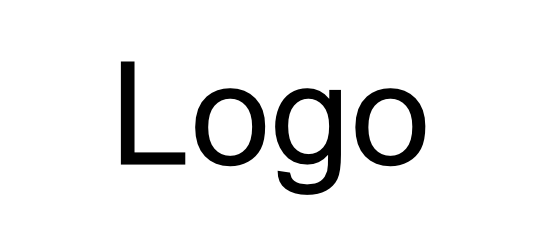
\includegraphics[scale=0.25]{dhbw-logo}};
\end{tikzpicture}

%Firmen Logo
\begin{tikzpicture}[remember picture,overlay]
 \node[anchor=north west,inner xsep=50pt, inner ysep=25pt] at (current page.north west)
 {
\includegraphics[scale=0.2]{company-logo}};
\end{tikzpicture}

%===========Inhalt===========================================
\vspace{0.5cm}

\begin{center}
 \large{\Titel}
\end{center}

\vspace{0.5cm}

\begin{center}
 \textbf{\Art}
\end{center}

\vspace{1.5cm}

\begin{center}
 des Studienganges \Studiengang \\
 an der Dualen Hochschule Baden-Württemberg Mannheim
\end{center}

\vspace{0.5cm}

\begin{center}
 von\\
 \Vorname{} \Nachname
\end{center}

\vspace{0.5cm}

\begin{center}
 \Abgabedatum
\end{center}

\vspace{0.5cm}

\begin{tabular}{l@{\hspace{2cm}}l}
 Bearbeitungszeitraum:            & \Bearbeitungszeitraum        \\
 Matrikelnummer, Kurs:            & \Matrikelnummer, \Kurskrzl   \\
 Ausbildungsfirma, Abteilung:     & \Ausbildungsfirma, \Abteilung\\
 Standort:                        & \Standort                    \\
 Betreuer der Ausbildungsfirma:   & \BetreuerFirma               \\
 Gutachter der Dualen Hochschule: & \BetreuerDHBW                \\
                                  
\end{tabular}


%List of Todos
\listoftodos\clearpage

%Sperrvermerk
\pagestyle{empty}
% !TeX root = ../../../template.tex
\chapter*{Sperrvermerk}
\glqq Der Inhalt dieser Arbeit darf weder als Ganzes noch in Auszügen Personen außerhalb des Prüfungsprozesses und des Evaluationsverfahrens zugänglich gemacht werden, sofern keine anders
lautende Genehmigung des Dualen Partners vorliegt.\grqq{} [Ende der Sperrfrist: \SperrvermerkAuslaufDatum]

% % !TeX root = ../../../template.tex
\chapter*{Sperrvermerk}
\addcontentsline{toc}{chapter}{Sperrvermerk}
Dieser Bericht enthält vertrauliche Daten der ABB Automation GmbH in Mannheim. Jegliche Vervielfältigung oder Veröffentlichung von Inhalten, Resultaten oder Zusammenfassungen ist nur mit ausdrücklicher schriftlicher Genehmigung der ABB Automation GmbH und unter Benachrichtigung des Autors gestattet.

\vspace{1.5cm}

\begin{tabularx}{0.9\textwidth}[b]{p{7cm} X p{7cm}}
\cline{1-1} \cline{3-3}
Ort, Datum &  & Unterschrift(Betreuer)
\end{tabularx}

%Der Inhalt dieser Arbeit darf weder als Ganzes noch in Auszügen Personen außerhalb des Prüfungsprozesses und des Evaluationsverfahrens zugänglich gemacht werden, sofern keine anders lautende Genehmigung des Dualen Partners vorliegt.
%[Ende der Sperrfrist: \SperrvermerkAuslaufDatum]


\pagenumbering{Roman}

%Eigenleistung
% !TeX root = ../../../template.tex
\chapter*{Erklärung}

Ich versichere hiermit, dass ich meine Bachelorarbeit mit dem
Thema: \Titel{} selbstständig verfasst und keine anderen als die angegebenen Quellen und Hilfsmittel
benutzt habe.
Ich versichere zudem, dass die eingereichte elektronische Fassung mit der gedruckten Fassung
übereinstimmt.\\\\\\\\
\begin{tabularx}{\textwidth}[b]{p{5cm} X p{5cm}} \cline{1-1} \cline{3-3}
 Ort, Datum &  & Unterschrift 
\end{tabularx}


%Abstract
% !TeX root = ../../template.tex
\chapter*{Abstract}
Die Firma \ac{p+f} ist im Bereich der Prozessautomation führender Hersteller für industrielle Sicherheitsausstattung. Das Produktportfolio umfasst eine Reihe industrieller Computersysteme für den Einsatz in explosionsgeschützten Bereichen. Durch den Einsatz in industriellen Umgebungen, sind diese Systeme Umwelteinflüssen wie Sonneneinstrahlung oder Vibrationen ausgesetzt. Durch eine falsche Abschätzung dieser Umwelteinflüsse können schädliche und unzulässige Betriebe entstehen. Oftmals können diese Betriebe nicht wahrgenommen werden. Um diesem Problem entgegenzuwirken, soll die in den Systemen verbaute Sensorik verwendet werden, um auf eben solche Betriebe hinzuweisen.\\
Diese Arbeit befasst sich im ersten Teil mit der Erarbeitung eines Konzepts, so wie einer Architektur für eine solche Health Monitoring Lösung für die \acl{p+f} \ac{hmi}-Plattformen. Dabei wird eine Architektur geschaffen, welche es ermöglicht plattformunabhängig Sensorwerte auszulesen und zu speichern. Des Weiteren wird ein Modell zur Zustandsbewertung der Plattformen definiert.\\
Im zweiten Teil dieser Arbeit wird ein Prototyp der Anwendung implementiert. Diese liest Sensoren der Plattformen aus, bewertet anhand der ausgelesenen Daten den Zustand des Gerätes und stellt die Daten eine Netzwerk-Schnittstelle bereit.
Zur Visualisierung der Daten wir zudem ein Dashboard erstellt, welches dezentral auf einem separaten Rechner bereitgestellt wird. In diesem können Sensordaten der Plattformen in Echtzeit abgerufen und präsentiert werden. 
% % !TeX root = ../../template.tex
\chapter*{Abstract}
The company \ac{p+f} is a leading manufacturer of industrial safety equipment in the field of process automation. The product portfolio includes a range of industrial computer systems for use in explosion-proof areas. Due to their use in industrial environments, these systems are exposed to environmental influences such as solar radiation or vibrations. An incorrect assessment of these environmental influences can result in harmful and unacceptable operations. Often these operations cannot be perceived. To counteract this problem, the sensor technology installed in the systems is used to indicate just such operations.\\
The first part of this thesis deals with the development of a concept and an architecture for such a health monitoring solution for the \acl{p+f} \ac{hmi} platforms. Thereby, an architecture is created, which allows platform-independent reading and storing of sensor values. Furthermore, a model for the state evaluation of the platforms is defined.
In the second part of this thesis a prototype of the application is implemented. It reads sensors of the platforms, evaluates the state of the device based on the read data and provides the data to a network interface.
For the visualization of the data a dashboard is created, which is provided decentralized on a separate computer. In this dashboard, sensor data from the platforms can be retrieved in real time.

%===================================================
%Verzeichnisse: Verwendete Verzeichnisse Aktivieren durch entfernen von: % vor dem \

%Inhaltsverzeichnis
\addcontentsline{toc}{chapter}{Inhaltsverzeichnis}\tableofcontents\clearpage

%Abbildungsverzeichnis
\addcontentsline{toc}{chapter}{Abbildungsverzeichnis}\listoffigures\clearpage

%Tabellenverzeichnis
\addcontentsline{toc}{chapter}{Tabellenverzeichnis}\listoftables\clearpage

%Lstingverzeichnis
% \addcontentsline{toc}{chapter}{Listingverzeichnis}\lstlistoflistings\clearpage

%Abkürzungsverzeichnis
% Wichtig, damit man nicht immer von Vorlage.tex bauen muss
% !TEX root = ../Vorlage.tex

\chapter*{Abkürzungsverzeichnis}
\begin{acronym}[slmtA]
    \acro{p+f}[P+F]{Pepperl+Fuchs}
    \acro{hmi}[HMI]{Human-Machine-Interface }
    \acro{sql}[SQL]{Structured Query Language}
    \acro{sequel}[SEQUEL]{Structured Englisch Query Language}
\end{acronym}

%===============================================================================

%Vorwort: Um Vorwort zu verwenden, % entfernen
% % !TeX root = ../../template.tex
\chapter*{Vorwort}
Hier kannst du dein Vorwort hinschreiben.


\pagestyle{scrheadings}
\pagenumbering{arabic}
%===============================================================================

%Eigene Kapitel
%Kapitel als eigene .tex datei erstellen und einbinden mit: \include{Pfad/Dateiname}
%% !TeX root = ../template.tex

\chapter{Beispiel Kapitel}
Die Datei zu diesem Kapitel findest du im Sections Ordner, als Example.tex.\\
In dieser Datei geht es darum euch einen Einblick in die Verwendung der Kommandos aus der Dokumentation Kapitel 3 zu geben \footcite{doku}.

\section{Aufzählungen}
Dort wird gezeigt wie man eine Aufzählung macht:
\begin{itemize}
 \item Erster Stichpunkt
 \item Zweiter Stichpunkt
\end{itemize}
Oder auch wie diese Nummeriert dargestellt werden können.
\begin{enumerate}
 \item Erster Stichpunkt
 \item Zweiter Stichpunkt
\end{enumerate}

\section{Bilder}
Zudem wird gezeigt wie man Bilder einfügt und diese referenzieren kann.
\begin{center}
 \begin{figure}[h!]
  \centering
  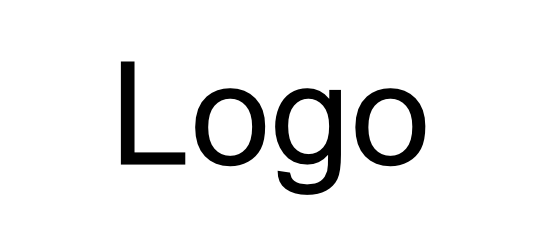
\includegraphics[scale = 0.3]{dhbw-logo}
  \caption{Dies ist ein Logo, link zu DHBW Logo ist in Pictures/downloads.txt zu finden}
  \label{fig:dhbwlogo}
 \end{figure}
\end{center}
Sowie zum Beispiel \ref{fig:dhbwlogo} referenziert wird.

\section{Zitieren}
Ein weiterer Teil ist, wie zitiert wird, ob auf \glqq{}Deutsche\grqq{} oder auf ``Englische'' Art und Weise\footcite[3.2]{doku}.

\cite[1]{doku}

\cite[1\psq]{doku}

\cite[1\psqq]{doku}

\cite[1-4]{doku}

\todo[inline]{Der Absatz-Stil sieht scheiße aus. Vorschag: parskip=full}

\section{Code}
\lstinline$var myValue$

You can write normal text and inbetween \lstinline$comes the inline listing aka code snippet$. Afterwards you can just continue writing normal text.

\begin{lstlisting}[caption={My caption}, label={lst:my-label-1}]
    import numpy as np
\end{lstlisting}

\lstinputlisting[caption={Here comes the caption},
                label={lst:my-label-2}]
                {resources/code/placeholder.py}

\chapter{Einleitung}
%\vspace{-1.2cm}\todo{eventuel einfach löschen}
%Im folgenden Kapitel wird die Grundlage für die vorliegende Bachelorarbeit geschaffen. Hierbei werden die Motivation und das Ziel der Arbeit erläutert, um einen klaren Überblick über den Themenkontext zu bieten. Des Weiteren werden die Anforderungen an das System gestellt.

\section{Pepperl + Fuchs / HMI}\label{sec:PFHMI}
Die Firma \ac{p+f} wurde 1945 von Walter Pepperl und Ludwig Fuchs gegründet. Anfangs war sie eine Radioreparaturwerkstadt, welche sich erst nach der Entwicklung eines eigenen Näherungsschalters so wie eines eigensicheren Transistorverstärkers auf das Gebiet der Elektronik ausweitete. Inzwischen entwickelt, produziert und vertreibt \ac{p+f} Baugruppen und Sensoren für den Automatisierungsmarkt. \cite{PFGeschichte}\\
\vspace{-1cm}
\begin{flushleft}
    \begin{figure}[h!]
        \centering
        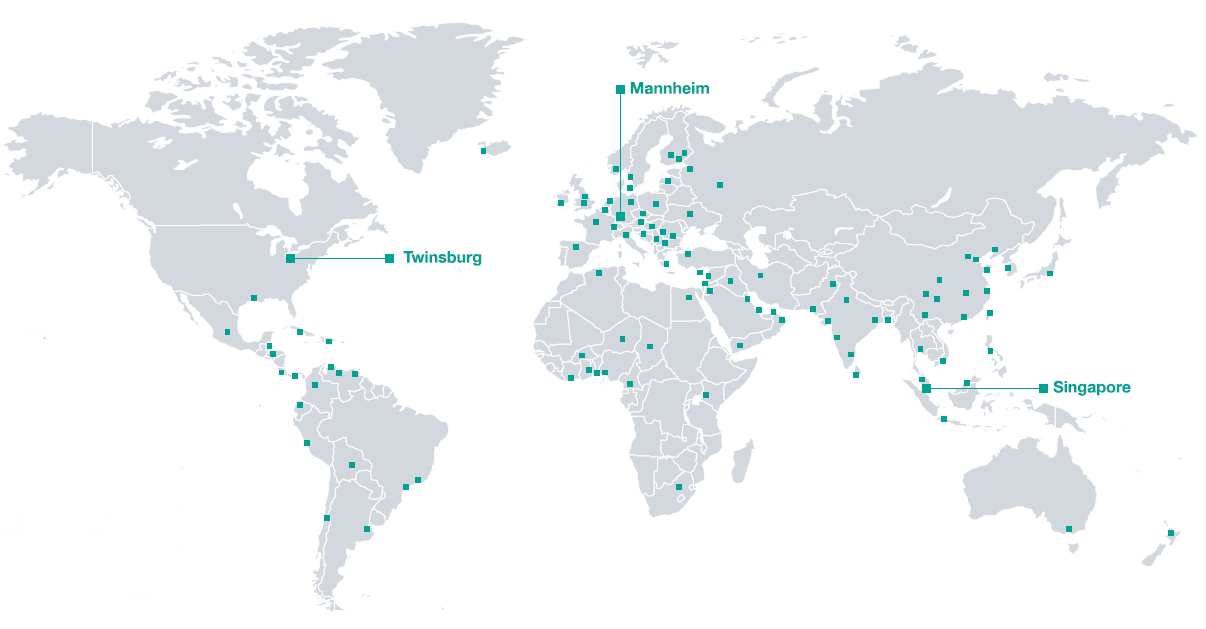
\includegraphics[width=1\linewidth]{P+F_Standorte.png}
        \caption{Standorte der Pepperl+Fuchs SE}
        \label{fig:StandortePF}
    \end{figure}
\end{flushleft}
Im Bereich der Prozessautomation ist \ac*{p+f} führender Hersteller industrieller Sicherheitsausstattungen. Das Produktportfolio umfasst eine Reihe von industrieller Computersysteme, welche zur Überwachung und Steuerung von Prozessen in explosionsgefährdeten Bereichen genutzt werde. Die \ac{hmi} Abteilung beschäftigt sich mit der Entwicklung dieser Systeme, welche eine Schnittstelle zwischen Mensch und Maschine bilden. Da es eine Vielzahl an Anwendungen für \ac{hmi} Systeme im explosionsgefährdeten Bereichen gibt, wurde die Produktfamilie \textit{VisuNet} speziell für den Einsatz in diesen Zonen konzipiert. Solche Ex-Zonen sind überall da zu finden, wo explosionsgefährliche Stoffe gelagert oder gehandhabt werden. In diesen Zonen kann durch Gas oder Staub, eine explosionsfähige Atmosphäre entstehen. Zudem kommen auch umwelttechnische Einflüsse wie Sonne, Nässe, Hitze und Kälte, aber auch Einflüsse, welche beispielsweise durch die Reinigung mit aggressiven Chemikalien entstehen, hinzu. Um in einen solchen Computer feindlichen Umgebung dennoch ein Prozessleitsystem zu integrieren, setzte \ac{p+f} mit den \textit{VisuNet} Remote Monitoren auf die Thin-Client-Technologie. Hierbei verbindet sich der Ex-Geschützte Monitor aus der Explosionsgefährdeten Zone mit der Zentralen, meist leistungsstärkeren, Recheneinheit in der No-Ex-Zonen. Eingaben über Tastatur und Maus werden anschließend über den Monitor an die Zentrale Recheneinheit weitergeleitet, welche anschließend die neuen Ausgaben an den Monitor zurückschickt. \cite{HMIYannick}

\section{Intention und Ziel der Arbeit}\label{sec:IZA}
Durch die Ex-Schutzzertifizierung der \textit{VisuNet} Plattformen, sind vorgeschriebene Betriebstemperaturgrenzen der Systeme einzuhalten. Integrierte Schutzschaltungen und weitere Sicherheitsmechanismen hindern die Geräten daran, diese Grenzwerte zu überschreiten. Umwelteinflüsse, wie beispielsweise die Sonneneinstrahlung oder Vibrationen, der industriellen Umgebungen in welchen die Geräte operieren, können negative Auswirkung auf die Systeme haben. Zudem können solche Umwelteinflüsse, Gerät in Systemzustände bringen, welche den Zertifizierungsrichtlinien widersprechen. Durch eine falsche Einschätzung der Umweltfaktoren werden unzulässige bzw. schädliche Betriebe vom Endkunden meist nicht wahrgenommen.\\
Eine Möglichkeit dem zu begegnen, ist die auf der Hardware verbaute Sensorik zu nutzen, um den Zustand des Systems zu überwachen. Aus den Daten können anschließend Rückschlüsse, auf Betriebszustände und das daraus resultierenden Nutzungsverhalten gezogen werden. Dem Nutzer können somit wichtige Informationen zum Systemzustand vermittelt werden, sodass schädliche bzw. kritische Zustände entdeckt und vermieden werden können.\\
Primäres Ziel dieser Bachelorarbeit ist daher, die prototypische Entwicklung einer Hardware-Health Monitoring Lösung für die \acl{p+f} \ac{hmi} Plattformen \textit{VisuNet GXP} und \textit{FLX}. Hierbei soll eine Architektur und Konzepterweiterung für den Aufbau einer verteilten Health-Monitoring Lösung, welche möglichst plattformunabhängig ausgeführt werden kann, erstellt werden. Dazu gilt es Sensoren und Messwerte, welche bei der„Health“- Status Definition berücksichtigt werden sollen, auszuwählen und auszulesen. Des Weiteren soll ein Modell definiert werden, welches die Sensor-Messwerte in einen plattformspezifischen Health-Status übersetzt, um dem Benutzer den aktuellen Zustand (Ampel-Prinzip) mitzuteilen. Als prototypische Umsetzung soll ein Health Agent, entwickelt werden, welche Geräte-Daten (z.B. aktuelle Temperatur) der \ac{hmi} Systeme ausliest, abspeichert, in der VisuNet RM Shell 6 dem Benutzer visualisiert und per Netzwerkprotokoll (z.B. MQTT oder SNMP) einem zentralen Server bereitstellen kann.    

\section{Anforderungen}\label{sec:Anforderungen}\todo{Anforderungen etwas mehr ausformulieren}
Durch das in Abschnitt \ref{sec:IZA} erläuterte Ziel dieser Arbeit, ergeben sich die unten aufgelisteten Anforderungen.
\begin{enumerate}
    \item Schnittstelle zur Datenerfassung
    \begin{enumerate}
        \item Auslesen der Systemsensorik\\
        Das System benötigt eine zentrale Schnittstelle, welche das Auslesen der Sensoren der VisuNet Plattformen ermöglicht. Die \textit{VisuNet} Plattformen unterscheiden sich in der ausgestatteten Elektronik so weit, dass verschiedene Ansätze zum Auswerten dieser benötigt werden. 
        \item Speichern der ausgelesenen Messwerte\\
        Zur Verwaltung der gesammelten Daten benötigt das System eine zentrale Datenbank. Diese muss über eine übersichtliche und effiziente Struktur verfügen, welche das Verarbeiten der gesammelten Daten im Nachgang ermöglicht.
    \end{enumerate}
    
    \item Datenverarbeitung
    \begin{enumerate}
        \item Ermittelung des Health Status\\
        Für die jeweiligen \textit{VisuNet} Plattformen soll der System Health Status ermittelt werden. Dieser soll eine Aussage über den Betrieb des Systems geben. 
        \item Ermittelung der Health Status Historie\\
        Über die gesammelten Health Status Daten soll zudem eine Historie erstellt werden. Diese soll eine Aussage über das generelle Nutzungsverhalten des Systems treffen. 
        \item Ermittelung der System Reliability\\
        Zudem soll eine Aussage über den Zustand des Systems, mittels Reliability, getroffen werden. 
    \end{enumerate}

    \item Datendistribution
    \begin{enumerate}
        \item Visualisierung der Systemdaten\\
        Die gesammelten Daten des Systems sollen über ein Dashboard visualisiert werden. In diesem soll dem Kunden, eine Auswertung des Systemverhaltens präsentiert werden. 
        \item Distribution der Daten zu einem externen Service\\
        Die gesammelten Daten des Systems sollen über ein Netzwerkprotokoll (MQTT, SNMP) an einen dritten Service übermittelt werden können.
    \end{enumerate}

   \end{enumerate}


%\chapter{Stand der Technik}

\section{Vergleich von Computer Monitoring Software auf dem Markt}
\subsection{Computer Monitoring Software}
\subsection{HWiNFO}

\section{VisuNetHardware}
\subsection{VisuNet FLX}
\subsection{VisuNet GXP}

\newpage

\section{Software Design Konzepte}
Eine solide Softwarerchitektur ist entscheidend für die erfolgreiche Entwicklung und Wartung eines Programmes. Sie legt den Grundstein für die anschließende Implementierung. Durch eine gute Architektur wird sichergestellt das das Programm Skalierbar, Effizient, Robust und gut zu warten ist.\\
Hierbei bieten sogenannte Design Patterns abhilfe. \textit{Jedes Muster beschreibt zunächst ein in userer Umwelt immer wieder auftretendes Problem, beschreibt dann den Kern der Lösung dieses Problems, und zwar so dass man diese Lösung milionenfach anwendden kann, ohne sich je zu wiederholen} (Christof Alexander \textit{Eine Muster-Sprache} [Löcker verlag, Wien, 1995, Seite x]). Diese definition für muster bezieht sich auch auf objektorientierte Design Patterns. Das verwenden dieser Patterns ermöglicht Entwicklern von der Erfahrung anderer zu profitieren, um bereits gelöste Probleme nicht nochmal lösen zu Müssen. Zudem steigern sie auch die Codequalität. Der Code wird Lesbarer und die Wartung dessen wird leichter. Zudem wird auch die Implementierung neuer Erweiterungen und das Eindenken in die Software durch gängige Designpatterns erleichtert. \cite[S.25 ff]{DesignPatterns}\\
\textit{Alle gut strukturierten objektorientierten Architekturen basieren auf Mustern} (Grady Booch \cite[S.21]{DesignPatterns}).
In den folgenden Kapiteln wird genauer auf die in dieser Arbeit verwendeten Design Patterns eingegangen.      

\subsection{Adapter Pattern}
Zweck des Adapter Patterns ist die Anpassung der Schnitstelle einer Klasse an eine andere von dem Client erwarteten Schnitstelle. Somit ermöglicht das Pattern die Zusammenarbeit von zwei Klassen, welche auf grund ihrer Schnellen nicht möglich wäre. Das Adapter Patern ist auch unter dem namen Wrapper bekannt, welcher im folgenden Verlauf der arbeit verwendet wird.\\
Das Pattern kommt immer dann zum einsatz, wenn eine bereits existierende Klasse genutzt werden soll, jedoch die Schnitstelle der klasse nicht mit den aktuellen Anforderungen des clients übereinstimmt. Desweiteren wird das Dattern verwendet, wenn eine wiederverwendbare Klasse erzeugt werden soll, welche mit unabhängigen und nocht vorhersehbaren Klassen interagieren soll.\\      
\begin{center}
    \begin{figure}[h]
     \centering
     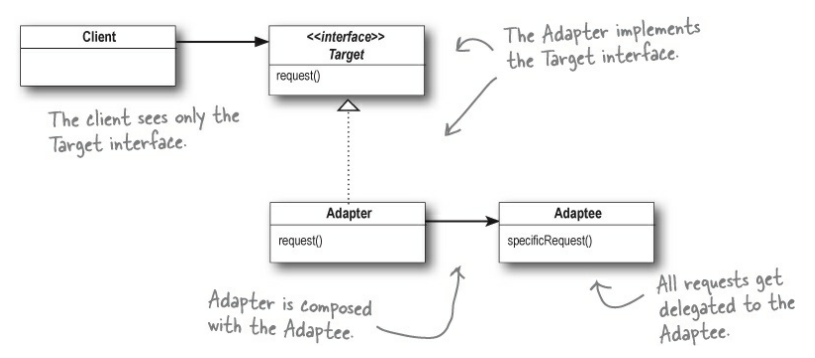
\includegraphics[width=1\linewidth]{UMLAdapterPattern}
     \caption{Adapter Pattern Struktur \cite{DesignPatterns}}
    \label{fig:AdapterPattern}
    \end{figure}
\end{center}
\vspace{-2cm}
Das Design Pattern besteht aus einem \textit{Target}, welches die vom Client verwendete Schnitstelle definiert. Zu dem kommt der \textit{Client}, welcher mit den Objekten zusammen arbeitet, die der Zielschnittstelle entsprechen. Zuletzt beinhaltet das Adapter Pattern einen \textit{Adaptee} so wie den \textit{Adapter} selbst. Der \textit{Adaptee} definiert eine bestehende Schnittstelle, welche vom \textit{Adapter} adaptiert werden muss.\\ 
Der \textit{Client} ruft die gewünschte Operation auf einer \textit{Adapter}-Instanz auf, welche anschließend die gewünschten \textit{Adaptee}-Operation ausführt.

\subsection{Strategie Design Pattern}
Zweck des Strategy (Strategie) Patterns ist es, eine Familie von einzelnen gekapselten und Austauschbaren Algorithmen zu schaffen. Dieses Patern ermöglicht eine variable und vom Client unabhöngige nutzung des Algorythmus.\\
Das Pattern kommt zum einsatz wenn eine Reihe von zusammenhängenden Klassen sich nur in Ihrem verhalten unterscheiden, verschiedene varianten eines Algorythmus erfordert werden, der Client keine Kenntnis von den vom Algorythmus verwendeten Daten haben soll, oder eine Klasse verschiedene Verhaltensweisen aufweist.\\
\begin{center}
    \begin{figure}[h]
     \centering
     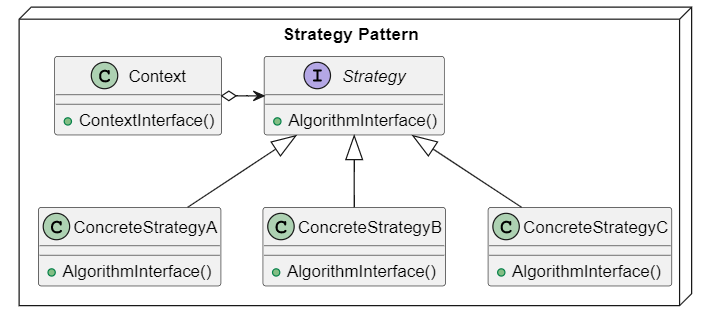
\includegraphics[width=1\linewidth]{UMLStrategyPattern}
     \caption{Strategie Pattern Struktur \cite{DesignPatterns}}
    \label{fig:StrategyPattern}
    \end{figure}
\end{center}
\vspace{-2cm}
Das Design Pattern besteht aus den folgenden Teilnehmern. Die \textit{Strategy}, welche eine gemeinsame Schnitstelle für die verwendeten Algorithmen deklariert. Einer oder mehreren \textit{ConcreteStrategy}, welche die Implementierung der Algorythmen oder Klassen ist, so wie dem \textit{Context}, welcher mit eier \textit{ConcreteStrategy} ausgestattet wird. Desweiteren bestitzt der \textit{Context} eine Referenz auf das \textit{Strategy} Objekt.\cite[S.383 ff]{DesignPatterns}\\
Über den \textit{Context} kann anschließend zur laufzeit des Programmes die benötigten \textit{ConcreteStrategy} geladen und ausgeführt werden. 
Ein konkretes Beispiel hierzu wird im buch \cite[Head First Design Patterns]{HeadfirstDesignPatterns} behandelt, was den nutzen dieses Patterns nochmal verdeutlicht. 

\section{Datenbanken}
Weltweit wurden im Jahr 2022 Daten im Umfang von 103.66 Zettabyte erfasst. Diese Zahl wird sich laut Statistik \ref{fig:DatenvolumenStatistik} bis zum Jahr 2026 verdoppelt haben. Angesicht dieser Zahlen, sind Datenbanken aus der heutigen Zeit nicht weg zu denken. Sie bieten eine Möglichkeit, große Mengen an Daten Strukturiert abzuspeichern und anschließend auszuwerten.\\
Hierbei werden Datenbanken Grundsätzlich in Zwei Kategorien unterteilt. Relatione Datenbank und "Nicht relatione Datenbanken". Unterschiede der Datenbankarten machen sich in der Sprache zum Auswerten der DB, ihrer Skalierbarkeit, der Struktur, der Eigenschaften und der Unterstützung durch die Comunity bemerkbar. 
\begin{center}
    \begin{figure}[h]
     \centering
     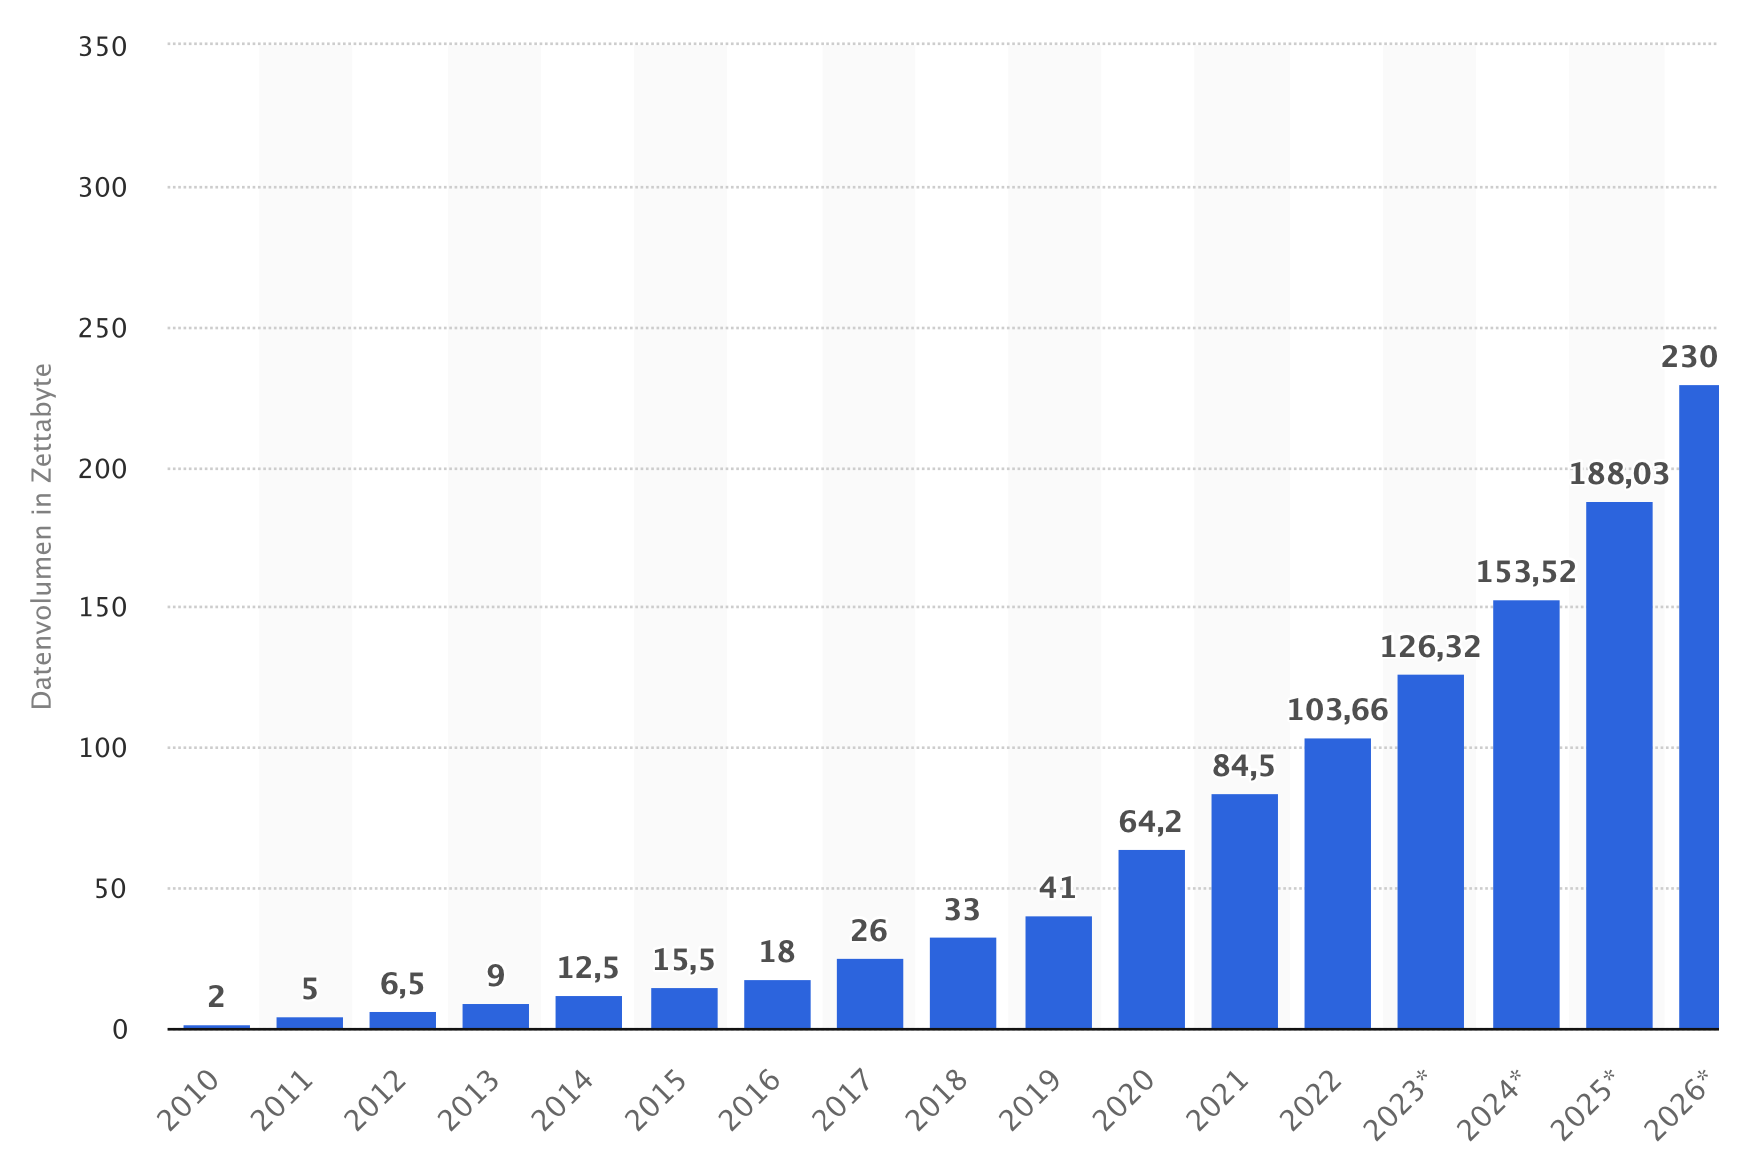
\includegraphics[width=1\linewidth]{DatenvolumenStatistik}
     \caption{Volumen der weltweit generierten Daten bis 2027 \cite{Datenmengen}}
    \label{fig:DatenvolumenStatistik}
    \end{figure}
\end{center}
\subsection{SQL - Structured Query Language}
IBM-Forscher Edgar F. Codd definierte 1969 ein Datenbankmodell für Relationale Datenbanken. Auf grundlagen seiner Forschung began, in den folgenden Jahren, die entwicklung der Sprache \ac{SEQUEL}. Codds Modell für bassiert auf der zuordnung von Schlüsseln. Nach einigen Überarbeitungen der implementierung wurde diese anschließend in \ac{SQL} umbenannt.\\
\ac{SQL} ermöglicht insbesondere die Speicherung, Bearbeitung so wie eine Abfrage von Daten in einer Datenbank. Mithilfe des Prinzips der Schlüssel, können Datensätze miteinander verknüpft werden. Somit kann einem Benutzernamen bespielsweise ein echter Name, eine Telefonnummer und eine Email-Addresse zugewiesen werden.\\
Die besondere eigenschaft von \ac{SQL} ist das Konzepte von Arrays. Relationale Datenbanken bestehen aus Arrays, welche sich mit Hilfe von verschiedenen Befehen erzeugen und bearbeiten. \cite{SQL}\\
\ac{SQL} beitet eine reihe von Befehlen, welche die Interaktion mit der Datenbank ermöglichen. Diese können Grundsätzlich in 5 Kategorien eingeteilt werden (siehe Abb. \ref{fig:SQLCommands}). Die wichtigsten Befehle sind dabei \text{INSERT}, \textit{UPDATE} und \textit{DELEAT}, mit welchen sich datensätze schreiben und bearbeiten lassen. Zudem der kommt der \textit{SELECT} Befehl, welcher das auslesen von Datensätzen ermöglicht. Um die tabellenstruktur der Datenbank zu berarbeiten kommen die Befehle \textit{CREATE} und \textit{DROP} zum einsatz. \cite{SQLCommands}\\
Natürlich bietet die Programmiersprache eine weit aus komplexere Sysntax, um datensätze sortiet auswerten zu könen. Eine vollständige dokumentation der Sprache findet sich auf der w3school webseite \cite{SQLDoku}.
\begin{center}
    \begin{figure}[h!]
     \centering
     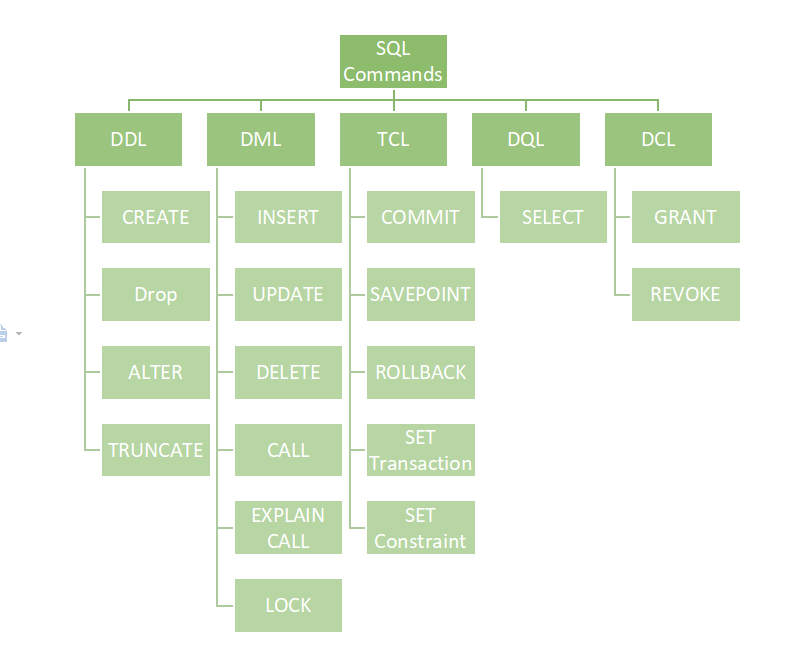
\includegraphics[scale = 0.3]{SQLCommands}
     \caption{SQL Befehls Kategorien \cite{SQLCommands}}
    \label{fig:SQLCommands}
    \end{figure}
   \end{center}

\subsection{SQLite Embedded Datenbank}
In der Vorarbeit zu dieser Bachelorarbeit wurde bereits eine auswahl für eine Datenbank getroffen. Dabei wurde sich nach einigen vergleichen für die SQLite Embedded Datenbank Engine entschieden. \\
Diese Bietet eine zuverlässige, kleine, schnelle und vollfunktionale Datenbank Engine, welche vollständige in das Gesamtsystem integriert werden kann \cite{SQLiteHompage}. Zur implementierung der Datenbank in die anwendung wird edie System.Data.SQLite bibliothek für C\# verwendet.\\

\section{MTBF und Reliability}


\section{Fuzzy Logic}

\section{Grafana}

%Grundlagen Kappitel
\chapter{Stand der Technik}
In diesem Kapitel werden die in dieser Arbeit verwendeten Konzepte und Technologien beleuchtet. 

\section{Vorarbeiten zur Bachelorthesis}
Zum Thema dieser Bachelorarbeit wurden bereits zwei Vorarbeiten geleistet. Zum einen wurde im Rahmen einer Praxisphase, eine Voruntersuchung zum Thema \textit{Condition-Based-Monitorig für industrielle PCs}  vorgenommen. Die im Rahmen dieser Arbeit \cite{PAMathias} durchgeführte Grundlagenuntersuchung und Marktrecherche hat auf zwei Computer Monitoring Technologien aufmerksam gemacht. Diese wurden anschließend in der zweiten Vorarbeit \cite{t3000} evaluiert. Aus dieser Bewertung heraus, wurde sich für die \textit{HWiNFO} Software, zum Auslesen der auf der Hardware verbauten Sensoren entschieden. Die Software wird genauer in Abschnitt \ref{sec:HWiNFO} behandelt. Des Weiteren wurde in der Vorarbeit \cite{t3000} auch eine geeignete Datenbank für das Health Monitoring System ausgewählt. In Abschnitt \ref{sec:SQLite} wird die ausgewählte Datenbanktechnologie genauer beschrieben. 

\subsection{SQLite Embedded Datenbank}\label{sec:SQLite}
In der Vorarbeit zu dieser Bachelorarbeit wurde bereits eine Auswahl für eine Datenbank getroffen. Hierbei wurden drei Datenbanken in den Punkten Performanz, Größe der Anwendung, Ressourcennutzung und der Dokumentation miteinander verglichen. Aus dem Vergleich hervorgehend, wurde sich anschließend für die Verwendung der SQLite Embedded Datenbank Engine entschieden. Diese bietet eine zuverlässige, kleine, schnelle und voll funktionale Datenbank Engine, welche vollständige in das Gesamtsystem integriert werden kann \cite{SQLiteHompage}. Zur Implementierung der Datenbank in die Anwendung wird die System.Data.SQLite Bibliothek für C\# verwendet.\\ 
Auf das Thema Datenbanken wird in Abschnitt \ref{sec:Datenbank} genauer eingegangen.

\subsection{HWiNFO}\label{sec:HWiNFO}
\textit{Hwinfo} ist eine Software der Firma REALiX, welche zum Überwachen und Analysieren der Hardware eines Computers konzipiert wird. Über die grafische Oberfläche des Programms, lassen sich alle gesammelten Daten anzeigen. Der Nutzer kann diese Informationen nutzen, um Defekte an der Hardware zu erkennen.\\
Das ausschlaggebende Argument für die Nutzung der Software liegt in der \ac{api}. Über die Shared Memory Funktion der Software lassen sich alle Gerätedaten, die die Software auslesen kann über eine C\# Bibliothek auslesen. Hierzu muss die Funktion in den Einstellungen des Programms eingeschaltet werden. Da die 64 bit Version des Tools dies nur für einen Zeitraum von 12h erlaubt, wird für den Verlauf der Arbeit die 32-bit Version der Software verwendet. Zum anderen bietet der REALiX einen \ac{sdk} welcher alle Funktionen der Software in Form einer Bibliothek bereitstellt.\cite{HWINFO}\\
Im Verlauf der Arbeit wird die Shared Memory Funktion der Software für die prototypische Implementierung des Health Monitorig Systems genutzt.   
% \section{Produktfamilie VisuNet}
Die Zielhardware für das Healthmonitoring System sind die \ac{p+f} VisuNet FLX und GXP Platformen. Diese sind Bedien- und Beobachtungssystemen für den Einsatz in Explosionsgefährdete bereichen. Durch  

\subsection{VisuNet FLX \& GXP}

\subsection{VisuNet RM Shell \& Control Center}
\section{Software Design Konzepte}
Eine solide Softwarerchitektur ist entscheidend für die erfolgreiche Entwicklung und Wartung eines Programmes. Sie legt den Grundstein für die anschließende Implementierung. Durch eine gute Architektur wird sichergestellt das das Programm Skalierbar, Effizient, Robust und gut zu warten ist.\\
Hierbei bieten sogenannte Design Patterns abhilfe. \textit{Jedes Muster beschreibt zunächst ein in userer Umwelt immer wieder auftretendes Problem, beschreibt dann den Kern der Lösung dieses Problems, und zwar so dass man diese Lösung milionenfach anwendden kann, ohne sich je zu wiederholen} (Christof Alexander \textit{Eine Muster-Sprache} [Löcker verlag, Wien, 1995, Seite x]). Diese definition für muster bezieht sich auch auf objektorientierte Design Patterns. Das verwenden dieser Patterns ermöglicht Entwicklern von der Erfahrung anderer zu profitieren, um bereits gelöste Probleme nicht nochmal lösen zu Müssen. Zudem steigern sie auch die Codequalität. Der Code wird Lesbarer und die Wartung dessen wird leichter. Zudem wird auch die Implementierung neuer Erweiterungen und das Eindenken in die Software durch gängige Designpatterns erleichtert. \cite[S.25 ff]{DesignPatterns}\\
\textit{Alle gut strukturierten objektorientierten Architekturen basieren auf Mustern} (Grady Booch \cite[S.21]{DesignPatterns}).
In den folgenden Kapiteln wird genauer auf die in dieser Arbeit verwendeten Design Patterns eingegangen.      

\subsection{Adapter Pattern}
Zweck des Adapter Patterns ist die Anpassung der Schnitstelle einer Klasse an eine andere von dem Client erwarteten Schnitstelle. Somit ermöglicht das Pattern die Zusammenarbeit von zwei Klassen, welche auf grund ihrer Schnellen nicht möglich wäre. Das Adapter Patern ist auch unter dem namen Wrapper bekannt, welcher im folgenden Verlauf der arbeit verwendet wird.\\
Das Pattern kommt immer dann zum einsatz, wenn eine bereits existierende Klasse genutzt werden soll, jedoch die Schnitstelle der klasse nicht mit den aktuellen Anforderungen des clients übereinstimmt. Desweiteren wird das Dattern verwendet, wenn eine wiederverwendbare Klasse erzeugt werden soll, welche mit unabhängigen und nocht vorhersehbaren Klassen interagieren soll.\\      
\begin{center}
    \begin{figure}[h]
     \centering
     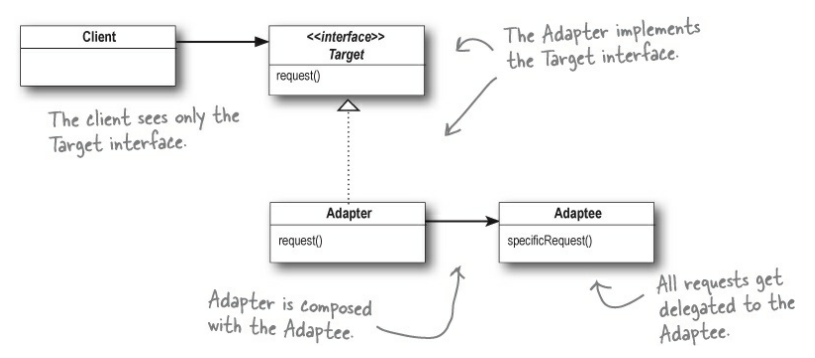
\includegraphics[width=1\linewidth]{UMLAdapterPattern}
     \caption{Adapter Pattern Struktur \cite{DesignPatterns}}
    \label{fig:AdapterPattern}
    \end{figure}
\end{center}
\vspace{-2cm}
Das Design Pattern besteht aus einem \textit{Target}, welches die vom Client verwendete Schnitstelle definiert. Zu dem kommt der \textit{Client}, welcher mit den Objekten zusammen arbeitet, die der Zielschnittstelle entsprechen. Zuletzt beinhaltet das Adapter Pattern einen \textit{Adaptee} so wie den \textit{Adapter} selbst. Der \textit{Adaptee} definiert eine bestehende Schnittstelle, welche vom \textit{Adapter} adaptiert werden muss.\\ 
Der \textit{Client} ruft die gewünschte Operation auf einer \textit{Adapter}-Instanz auf, welche anschließend die gewünschten \textit{Adaptee}-Operation ausführt.

\subsection{Strategie Design Pattern}
Zweck des Strategy (Strategie) Patterns ist es, eine Familie von einzelnen gekapselten und Austauschbaren Algorithmen zu schaffen. Dieses Patern ermöglicht eine variable und vom Client unabhöngige nutzung des Algorythmus.\\
Das Pattern kommt zum einsatz wenn eine Reihe von zusammenhängenden Klassen sich nur in Ihrem verhalten unterscheiden, verschiedene varianten eines Algorythmus erfordert werden, der Client keine Kenntnis von den vom Algorythmus verwendeten Daten haben soll, oder eine Klasse verschiedene Verhaltensweisen aufweist.\\
\begin{center}
    \begin{figure}[h]
     \centering
     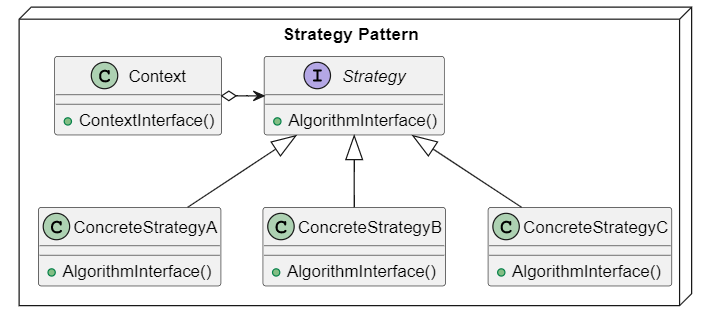
\includegraphics[width=1\linewidth]{UMLStrategyPattern}
     \caption{Strategie Pattern Struktur \cite{DesignPatterns}}
    \label{fig:StrategyPattern}
    \end{figure}
\end{center}
\vspace{-2cm}
Das Design Pattern besteht aus den folgenden Teilnehmern. Die \textit{Strategy}, welche eine gemeinsame Schnitstelle für die verwendeten Algorithmen deklariert. Einer oder mehreren \textit{ConcreteStrategy}, welche die Implementierung der Algorythmen oder Klassen ist, so wie dem \textit{Context}, welcher mit eier \textit{ConcreteStrategy} ausgestattet wird. Desweiteren bestitzt der \textit{Context} eine Referenz auf das \textit{Strategy} Objekt.\cite[S.383 ff]{DesignPatterns}\\
Über den \textit{Context} kann anschließend zur laufzeit des Programmes die benötigten \textit{ConcreteStrategy} geladen und ausgeführt werden. 
Ein konkretes Beispiel hierzu wird im buch \cite[Head First Design Patterns]{HeadfirstDesignPatterns} behandelt, was den nutzen dieses Patterns nochmal verdeutlicht.
\section{Datenbanken}\label{sec:Datenbank}
\begin{wrapfigure}{r}{0.5\textwidth}
    \vspace{-1.2cm}
    \captionsetup{justification=centering,format=plain, font=small}
    \begin{center}
      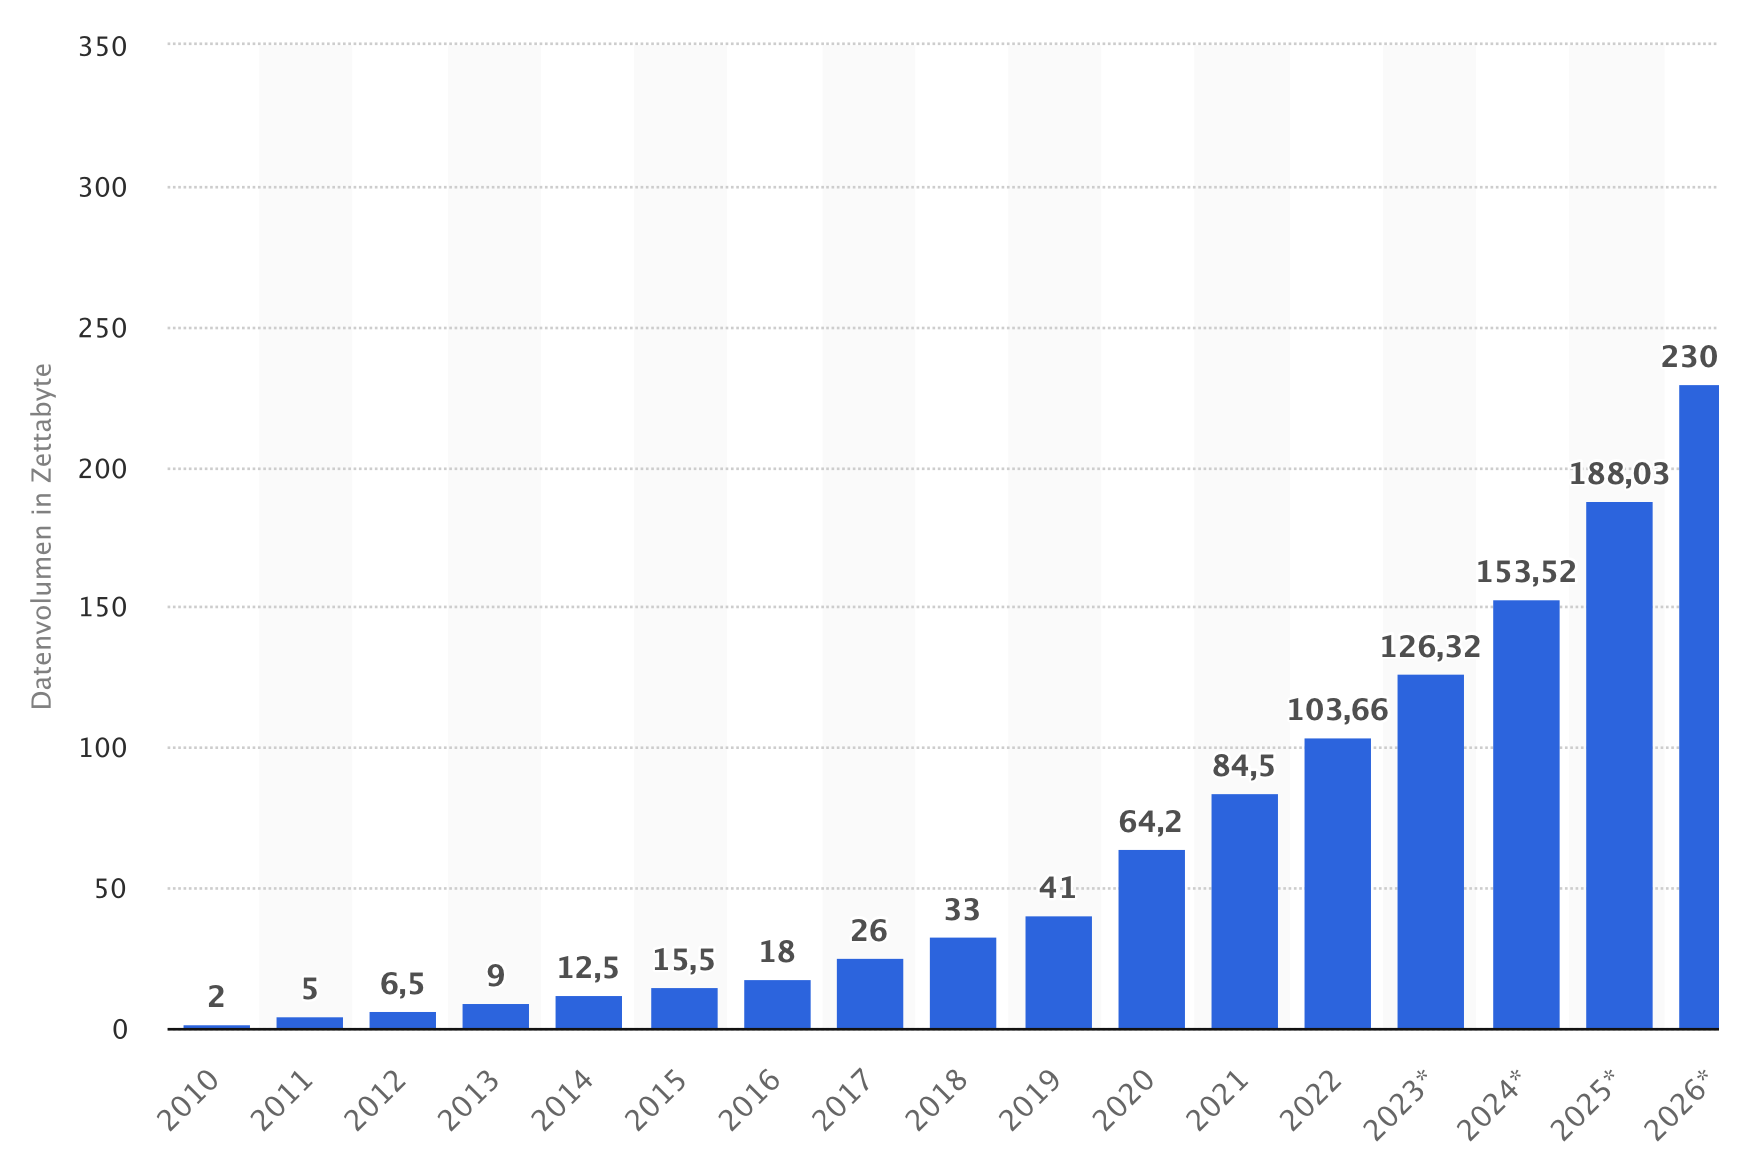
\includegraphics[width=0.48\textwidth]{DatenvolumenStatistik}
    \end{center}
    \vspace{-0.5cm}
    \caption{Volumen der weltweit generierten Daten bis 2027 \cite{Datenmengen}}
    \label{fig:DatenvolumenStatistik}
    \vspace{-0.5cm}
  \end{wrapfigure}
Weltweit wurden im Jahr 2022 Daten im Umfang von 103.66 Zettabyte erfasst \cite{Datenmengen}. Diese Zahl wird sich laut Statistik \ref{fig:DatenvolumenStatistik} bis zum Jahr 2026 verdoppelt haben. Angesichts dieser Zahlen, sind Datenbanken aus der heutigen Zeit nicht mehr wegzudenken. Sie bieten eine Möglichkeit, große Mengen an Daten strukturiert abzuspeichern und auszuwerten.\\
Hierbei werden Datenbanken grundsätzlich in zwei Kategorien unterteilt. Relationale und nicht relationale Datenbanken. Unterschiede der Datenbankarten machen sich in der Sprache zum Auswerten der Datenbank, ihrer Skalierbarkeit, der Struktur, der Eigenschaften und der Unterstützung durch die Community bemerkbar. \cite{SQLNoSQL} 

\subsection{SQL - Structured Query Language}
\begin{wrapfigure}{r}{0.5\textwidth}
    \vspace{-1.2cm}
    \captionsetup{justification=centering,format=plain, font=small}
    \begin{center}
      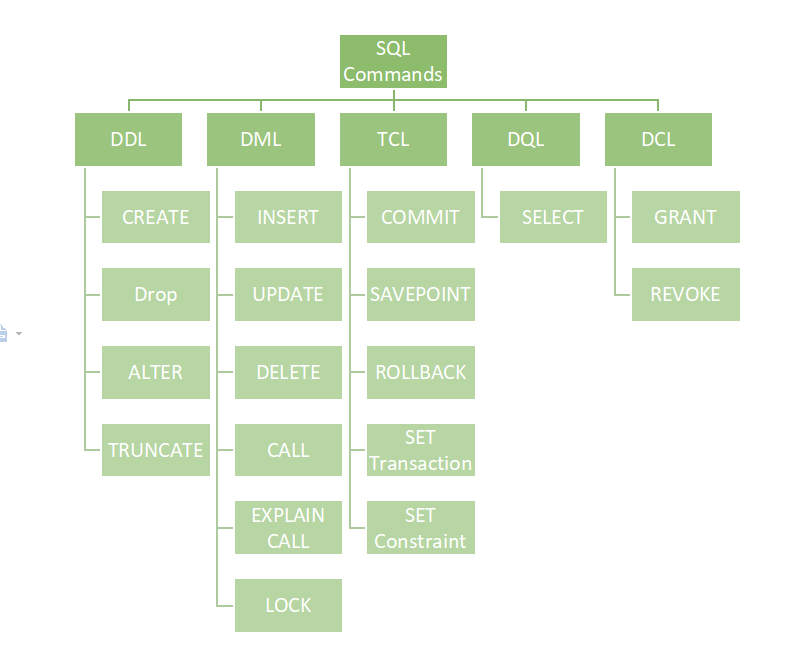
\includegraphics[width=0.48\textwidth]{SQLCommands}
    \end{center}
    \vspace{-0.5cm}
    \caption{SQL Befehls Kategorien \cite{SQLCommands}}
    \label{fig:SQLCommands}
    \vspace{-0.5cm}
  \end{wrapfigure}
IBM-Forscher Edgar F. Codd definierte 1969 ein Datenbankmodell für Relationale Datenbanken. Auf Grundlagen seiner Forschung begann in den folgenden Jahren die Entwicklung der Sprache \ac{sequel}. Codds Modell basiert auf der Zuordnung von Schlüsseln. Nach einigen Überarbeitungen der Implementierung wurde diese anschließend in \ac{sql} umbenannt.\cite{SQL}\\
\ac{sql} ermöglicht insbesondere die Speicherung, Bearbeitung sowie eine Abfrage von Daten in einer Datenbank. Mithilfe des Prinzips der Schlüssel können Datensätze innerhalb einer Datenbank miteinander verknüpft werden. Somit kann einem Benutzernamen beispielsweise ein echter Name, eine Telefonnummer und eine E-Mail Adresse zugewiesen werden.\cite{SQL}\\
Die besondere Eigenschaft von \ac{sql} ist das Konzept von Arrays. Relationale Datenbanken bestehen aus Arrays, welche sich mithilfe von verschiedenen Befehlen erzeugen und bearbeiten lassen.\cite{SQL}\\
\ac{sql} bietet dabei eine Reihe von Befehlen, welche die Interaktion mit der Datenbank ermöglichen. Diese können grundsätzlich in 5 Kategorien eingeteilt werden (siehe Abb. \ref{fig:SQLCommands}). Die wichtigsten Befehle sind dabei \textit{INSERT}, \textit{UPDATE} und \textit{DELEAT}, mit welchen sich Datensätze schreiben und bearbeiten lassen. Zudem kommt der Befehl \textit{SELECT}, welcher das Auslesen von bestimmten Datensätzen ermöglicht. Um die Tabellenstruktur der Datenbank zu bearbeiten, kommen die Befehle \textit{CREATE} und \textit{DROP} zum Einsatz.\cite{SQLCommands}\\
Natürlich bietet die Programmiersprache eine weitaus komplexere Syntax, um Datensätze sortiert auswerten zu können. Eine vollständige Dokumentation der Sprache findet sich auf der w3school Webseite \cite{SQLDoku}.
\section{MTBF und Reliability}\label{sec:MTBF}
Es gibt viele Ursachen, welche zu einem Ausfall elektronischer Komponenten in einem System, führen können. Laut dem technischen Bericht \cite{AIP} ist in 50\% der Fälle die Temperatur der Komponenten für einen Ausfall verantwortlich. Dies liegt an den unterschiedlichen thermischen Ausdehnungskoeffizienten des Materials auf der Platine haben. Durch die unterschiedliche Ausdehnung der Bauteile und der Platine selbst, kommt es zu hohen Belastungen der Lötstellen. Während sich dieser Zyklus wiederholt,  können Risse in den Verbindungen entstehen und ausbreiten. Diese können anschließend zu einem Bruch im elektrischen Stromkreis führen. \cite{AREPA_LifeExpectancy}\\
\begin{wrapfigure}{r}{0.65\textwidth}
    \vspace{-1.2cm}
    \begin{center}
      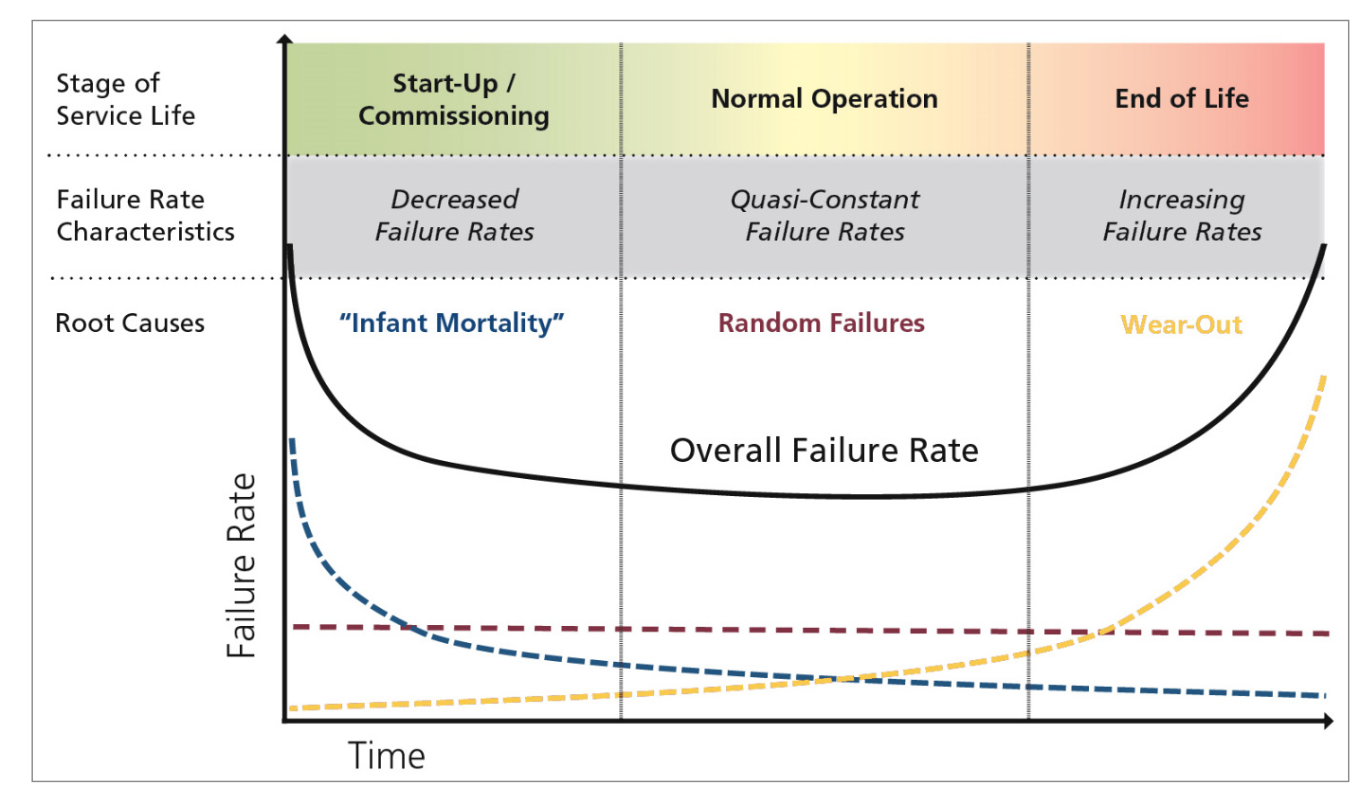
\includegraphics[width=0.64\textwidth]{BathTubCurve}
    \end{center}
    \vspace{-0.5cm}
    \caption{Bathtub Curve \cite{AREPA_LifeExpectancy}}
    \label{fig:BathTubCurve}
    \vspace{-0.5cm}
  \end{wrapfigure}
  Die in Abbildung \ref{fig:BathTubCurve} abgebildete Bathtub-Kurve ist ein Konzept, welches zur Beschreibung der Lebensdauer von elektronischer Komponenten verwendet wird. Dabei kann die Lebenszeit in drei Abschnitte unterteilt werden. Die Bathtub-Kurve beschreibt eine mittlere Betriebsdauer zwischen Ausfällen. Sie weist drei Betriebsphasen auf. 
  In der ersten Phase, bekannt als \textit{Infant Mortality}, kommt es durch Konstruktions-, Produktions- und Werkstoffmängel häufig gleich zu Beginn des Betriebs zu Fehlern und Ausfällen. Geräte, die von diesen Problemen nicht betroffen sind, laufen meist zuverlässig durch die zweite Phase der Kurve, bekannt als \textit{Random Failures}. Hierbei kommt es nur deutlich seltener und vereinzelt zu Ausfällen. Zum Ende der Lebensdauer kommt es, in der \textit{Wear-Out} Phase, durch Alterung und Verschleiß wieder vermehrt zu Ausfällen. \cite{AREPA_LifeExpectancy}\\ 
  Der \ac{mtbf} ist dabei eine statistische Kennzahl, die den durchschnittlichen Zeitraum in Stunden angibt, der zwischen zwei aufeinanderfolgenden Ausfällen einer bestimmten Komponente, eines Systems oder eines Produkts verstrichen is. Dieser weist zudem eine Temperaturabhängigkeit auf. Beispielsweise bei Kapazitäten kann im Durchschnitt gesagt werden: \textit{Eine Erhöhung der Betriebstemperatur um 10°C, führt zu einer Halbierung der Lebenserwartung}. Ein \ac{mtbf} von 100h sagt also aus, dass ein System im Durchschnitt, 100h laufen wird, bevor es zu einem Fehler kommen wird.\cite{MTBFReliability}\\
  Die Zuverlässigkeit (Reliability) eines Gerätes hingegen ist als die Wahrscheinlichkeit definiert, mit der ein System seine beabsichtigten Funktionen für einen festgelegten Zeitraum erfüllen wird. Hat ein System bei 100h eine Zuverlässigkeit von 0.8, so besteht eine 80\% Wahrscheinlichkeit, dass das System nach 100h noch funktioniert.\cite{MTBFReliability}\\
  Die Zuverlässigkeit eines Systems kann über den \ac{mtbf} mit Formel \ref{equ:Reliability} berechnet werden. Dabei ist zu beachten, dass man die Temperaturabhängigkeiten des Systems beachtet.
\begin{align}
    && R(t) &= e^{-\frac{t}{\text{mtbf}}} &&
    \label{equ:Reliability} 
\end{align}

\section{FuzzyLogic}
\section{Grafana}
Grafana ist eine Open-Source-Software zur plattformübergreifenden Analyse von Metriken und Daten. Als Webservice gehostet, ermöglicht es die Visualisierung von Daten mithilfe von vorgefertigten Vorlagen für Tabellen und Graphen. Diese Software unterstützt verschiedene Datenquellen und kann problemlos direkt mit einer relationalen Datenbanken verbunden werden. Grafana erleichtert somit die präzise Darstellung und Interpretation von Informationen durch benutzerfreundliche Visualisierungstools. \cite{GrafanaWebsite}\\
\vspace{-1cm}
\begin{center}
    \begin{figure}[h]
     \centering
     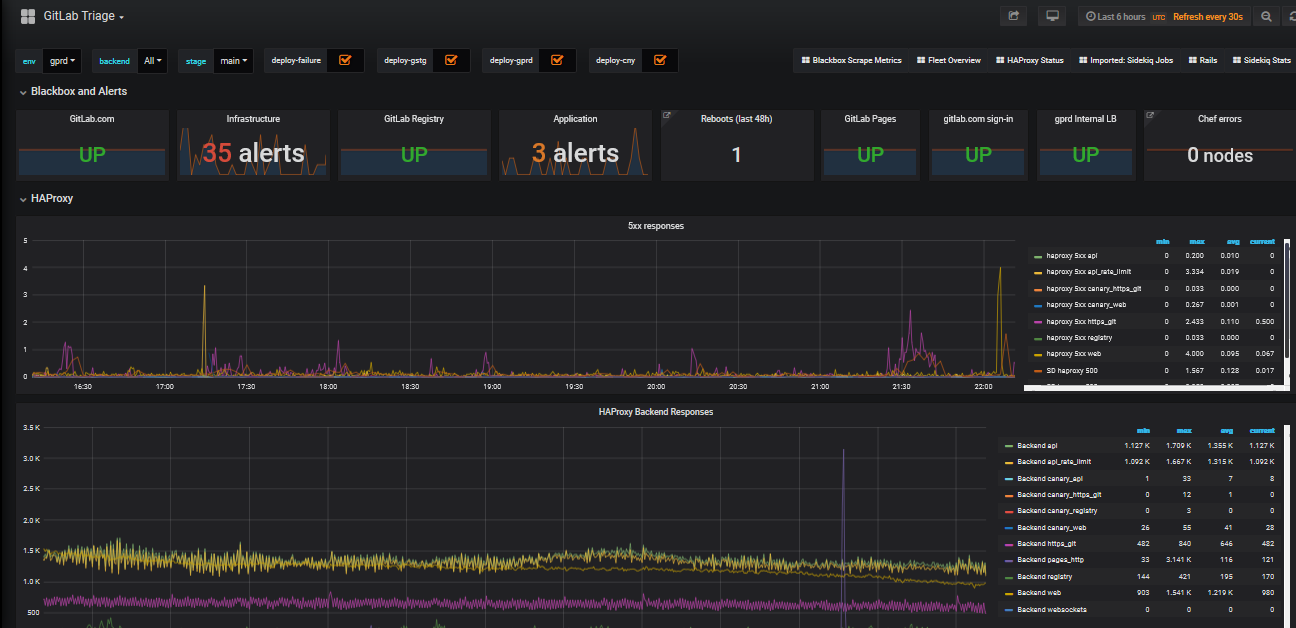
\includegraphics[width=0.8\textwidth]{Gitlab_Dashboard.png}
     \caption{Grafana Dashboard Beispiel \cite{GrafanaWebsite}}
     \label{fig:FuzzyLogicArchitektur}
    \end{figure}
   \end{center}


%System Architektur
\chapter{Architektur Konzept}
In diesem Kapitel wird die Struktur und Architektur der Hardware-Health-Monitroing Lösung erläutert. Die Architektur wird dabei zur Übersichltichkeit in drei Teilkomponenten unterteilt.\\
Abschnitt \ref{sec:Datenerfassung} befasst sich dabei mit der Datenerfassung. Hier wird das Konzept zum Plattform übergreifenden Auslesen der Hardwaresensorik und der Schpeicherung der erfasten Messdaten beleuchtet. In Abschnitt \ref{sec:Datenverarbeitung} wir anschließend das Modell zur bewertung des Systemzustnads erläutert.
Die Zusammenführung der einzelnen Teilsystem wird in Abschnitt \ref{sec:Gesamtkonzept} beschrieben. Zu letzt wird das Konzept zur Visualisierung der Daten in \ref{sec:Datenvisualisierung} beleuchtet. 
\section{Datenerfassung}\label{sec:Datenerfassung}
Die Herausforderung beim Auslesen der Daten liegt darin, die plattformspezifischen Informationen in einem allgemeinen Datenmodell zu konsolidieren. Hierbei stammen die Daten aus verschiedenen Schnittstellen. Die Architektur muss in der Lage sein, sämtliche verfügbaren Sensordaten plattformunabhängig auszulesen, darunter beispielsweise Temperaturen und CPU-Auslastung. Zusätzlich sollte sie die Integration weiterer plattformspezifischer Hardwarekonfigurationen und Schnittstellen ermöglichen, ohne eine grundlegende Neustrukturierung des bestehenden Codes zu erfordern.\\
Das Speichern der ausgelesenen Messdaten soll in einem einheitlichen Format erfolgen, das unabhängig von der Hardwarekonfiguration der Zielplatform ist. Zudem ist eine klare und sinnhafte Struktur der Datenbank wichtig, da diese Performant und Skalierbar sein muss.   

\subsection{Entwurf einer Architektur zum Auslesen der Systemhardware}\label{sec:AuslesenHardware}
 
Die Objekte und Klassen, die für das Auslesen der Systemhardware verwendet werden, sind im Verzeichnis \textit{HM.HWServices} abgelegt. Dieses Verzeichnis enthält alles, was benötigt wird, um die Hardware der Zielplatformen auszulesen.\\
Das UML Diagramm in Abbildung \ref{fig:HWServicesUML} veranschaulicht den Aufbau von \textit{HM.HWServices}. 
\begin{center}
    \begin{figure}[h!]
        \centering
        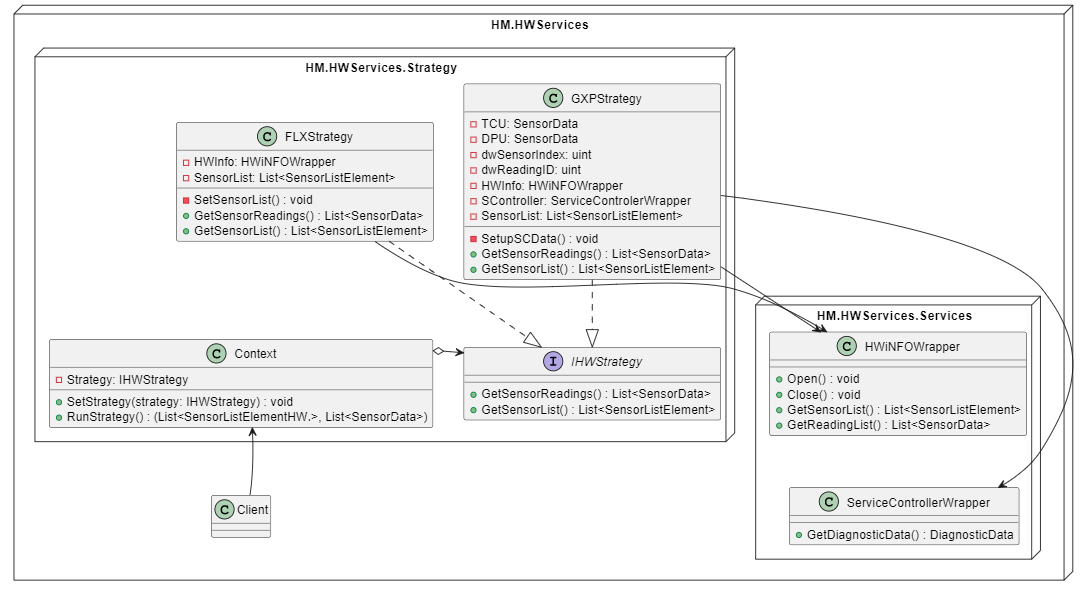
\includegraphics[width=1\textwidth]{UMLDatenerfassung.png}
        \caption{Architektur der HM.HWServices für das Auslesen der Hardware}
        \label{fig:HWServicesUML}
    \end{figure}
\end{center}
\vspace{-1.8cm}
Die Architektur der \textit{HM.HWServices} wird nach dem, in Abschnitt \ref{sec:StrategyPattern} beschriebnen Strategie Muster ausgelegt.
Die Komponenten des Strategie Musters sind im Verzeichnis \textit{HM.HWServices.Strategy} organisiert.\\
Durch den \textit{Context} kann die gewünschte Strategie ausgewählt und aufgerufen werden. Die Client-Anwendung interagiert dabei ausschließlich mit dem \textit{Context}, der wiederum die gewünschten Funktionen der ausgewählten Strategieklasse aufruft.\\  
Da sich das Auswerten von VisuNet FLX und GXP voneinander unterscheidet, soll für jede Platform eine eigene Strategieklasse verantwortlich sein. Jede dieser Strategieklasse wird hierbei von dem \textit{IHWStrategy} Interface abgeleitet. Dieses definiert die Struktur der Klassen, sodas die Funktion der ausgewählten Klasse im \textit{Context} ausgeführt werden kann, ohne die spezifische Strategieklasse genau zu kennen. Anschließend kann beim Start des Programms entschieden werden, welche dieser Strategien angewendet werden soll.\\
Muss das Programm in Zukunft um eine neue Hardwarekonfiguration einer Platform erweitert werden, kann dies über das hinzufügen einer weiteren Strategieklasse realisiert werden.\\
Zum Auslesen der Sensordaten stehen zunächst zwei Schnittstellen zurverfügung. Zum einen liefert über die in Abschnitt \ref{sec:HWiNFO} beschriebene Shared Memory Funktion der HWiNFO Software Messwerte aller an das Mainboard angeschlossenen Sensoren. Die VisuNet FLX Platform bedarf keiner weiteren Schnittstellen zum lesen von Sensordaten.\\
Um die Temperatursensoren in \ac{dpu} und \ac{tcu} der VisuNet GXP Plattform aus zu lesen, wird eine Weitere Bibliothek verwerwendet, welche die Komunikation mit dem in der Platform verbauten Servicecontroller ermöglicht.\\
Für beide Schnittstellen wurde eine Wrapperklasse (Siehe Abschnitt \ref{sec:AdapterPattern}) konzipiert, welche die wesentlichen Funktionen in einer übersichtlichen Klasse bereitstellen und die Datenstruktur der Schnittstelle adaptieren. Die Wrapperklassen werden im Verzeichnis \textit{HM.HWServices.Wrapper} organisiert. Die Wrapperklassen sind in Abbildung \ref{fig:HWServicesUML} zu sehen.
\subsubsection*{Adaption der Schnittstelle}
Beim Auslesen der Sensorik über die \textit{HWiNFOWrapper} Klasse, können zwei Listen ausgelesen werden. Zum einen werden alle verfügbaren Sensoren der Platform in einer Liste von \textit{SensorListElement} abgelegt. Zum anderen wird eine Liste des Typen \textit{SensorData} erzeugt. In dieser ist jeder Sensor mit dem aktuellen Messwertwert hinterlegt. Die Datentypen hierzu sind in Abbildung \ref{fig:DatastructuresUML} abgebildet.\todo{Mit UML der Wrapper erweitern}      
\begin{center}
    \begin{figure}[h!]
        \centering
        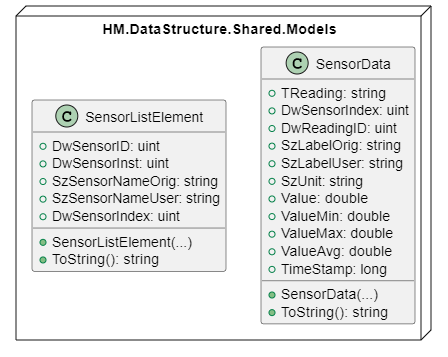
\includegraphics[width=0.45\textwidth]{UMLDatastructureHWI.png}
        \caption{Datenstruktur zum zwischenspeichern der Sensordaten}
        \label{fig:DatastructuresUML}
    \end{figure}
\end{center}
\vspace{-1.8cm}

\subsubsection*{Strategie Konzept}
Ziel der Strategieklassen ist wie zuvor bereits erwähnt die Kapselung der Algorithmen zum Auslesen der Zielplatformen. Eine Strategie soll daher folgende daten zurück liefern: Zum einen soll eine Aufzählung aller Sensoren im System erstellt werden, und in einer Liste von \textit{SensorListElement} hinterlegt werden. (Siehe Tabelle \ref{fig:SensorList}) 
\vspace{-0.5cm}
\begin{center}
    \begin{table}[h!]
        \centering
        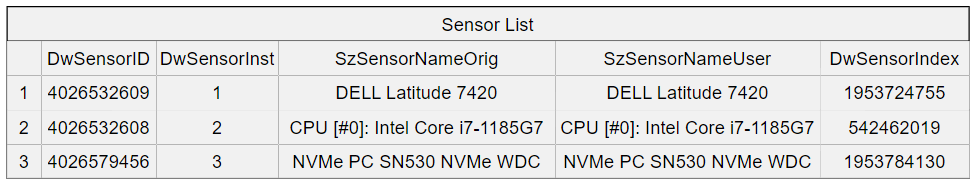
\includegraphics[width=0.7\textwidth]{SensorList.png}
        \caption{Beispiel einer Liste bestehend aus \textit{SensorListElement}}
        \label{fig:SensorList}
    \end{table}
\end{center}
\vspace{-1.8cm}
Zum anderen soll ein aktueller Auszug der Sensorwerte erstellt werden können. Hierzu sollen die Werte der einzelnen Sensoren in einer Liste von \textit{SensorData} gespeichert werden. (Siehe Tabelle \ref{fig:SensorReadings})
\vspace{-0.5cm}
\begin{center}
    \begin{table}[h!]
        \centering
        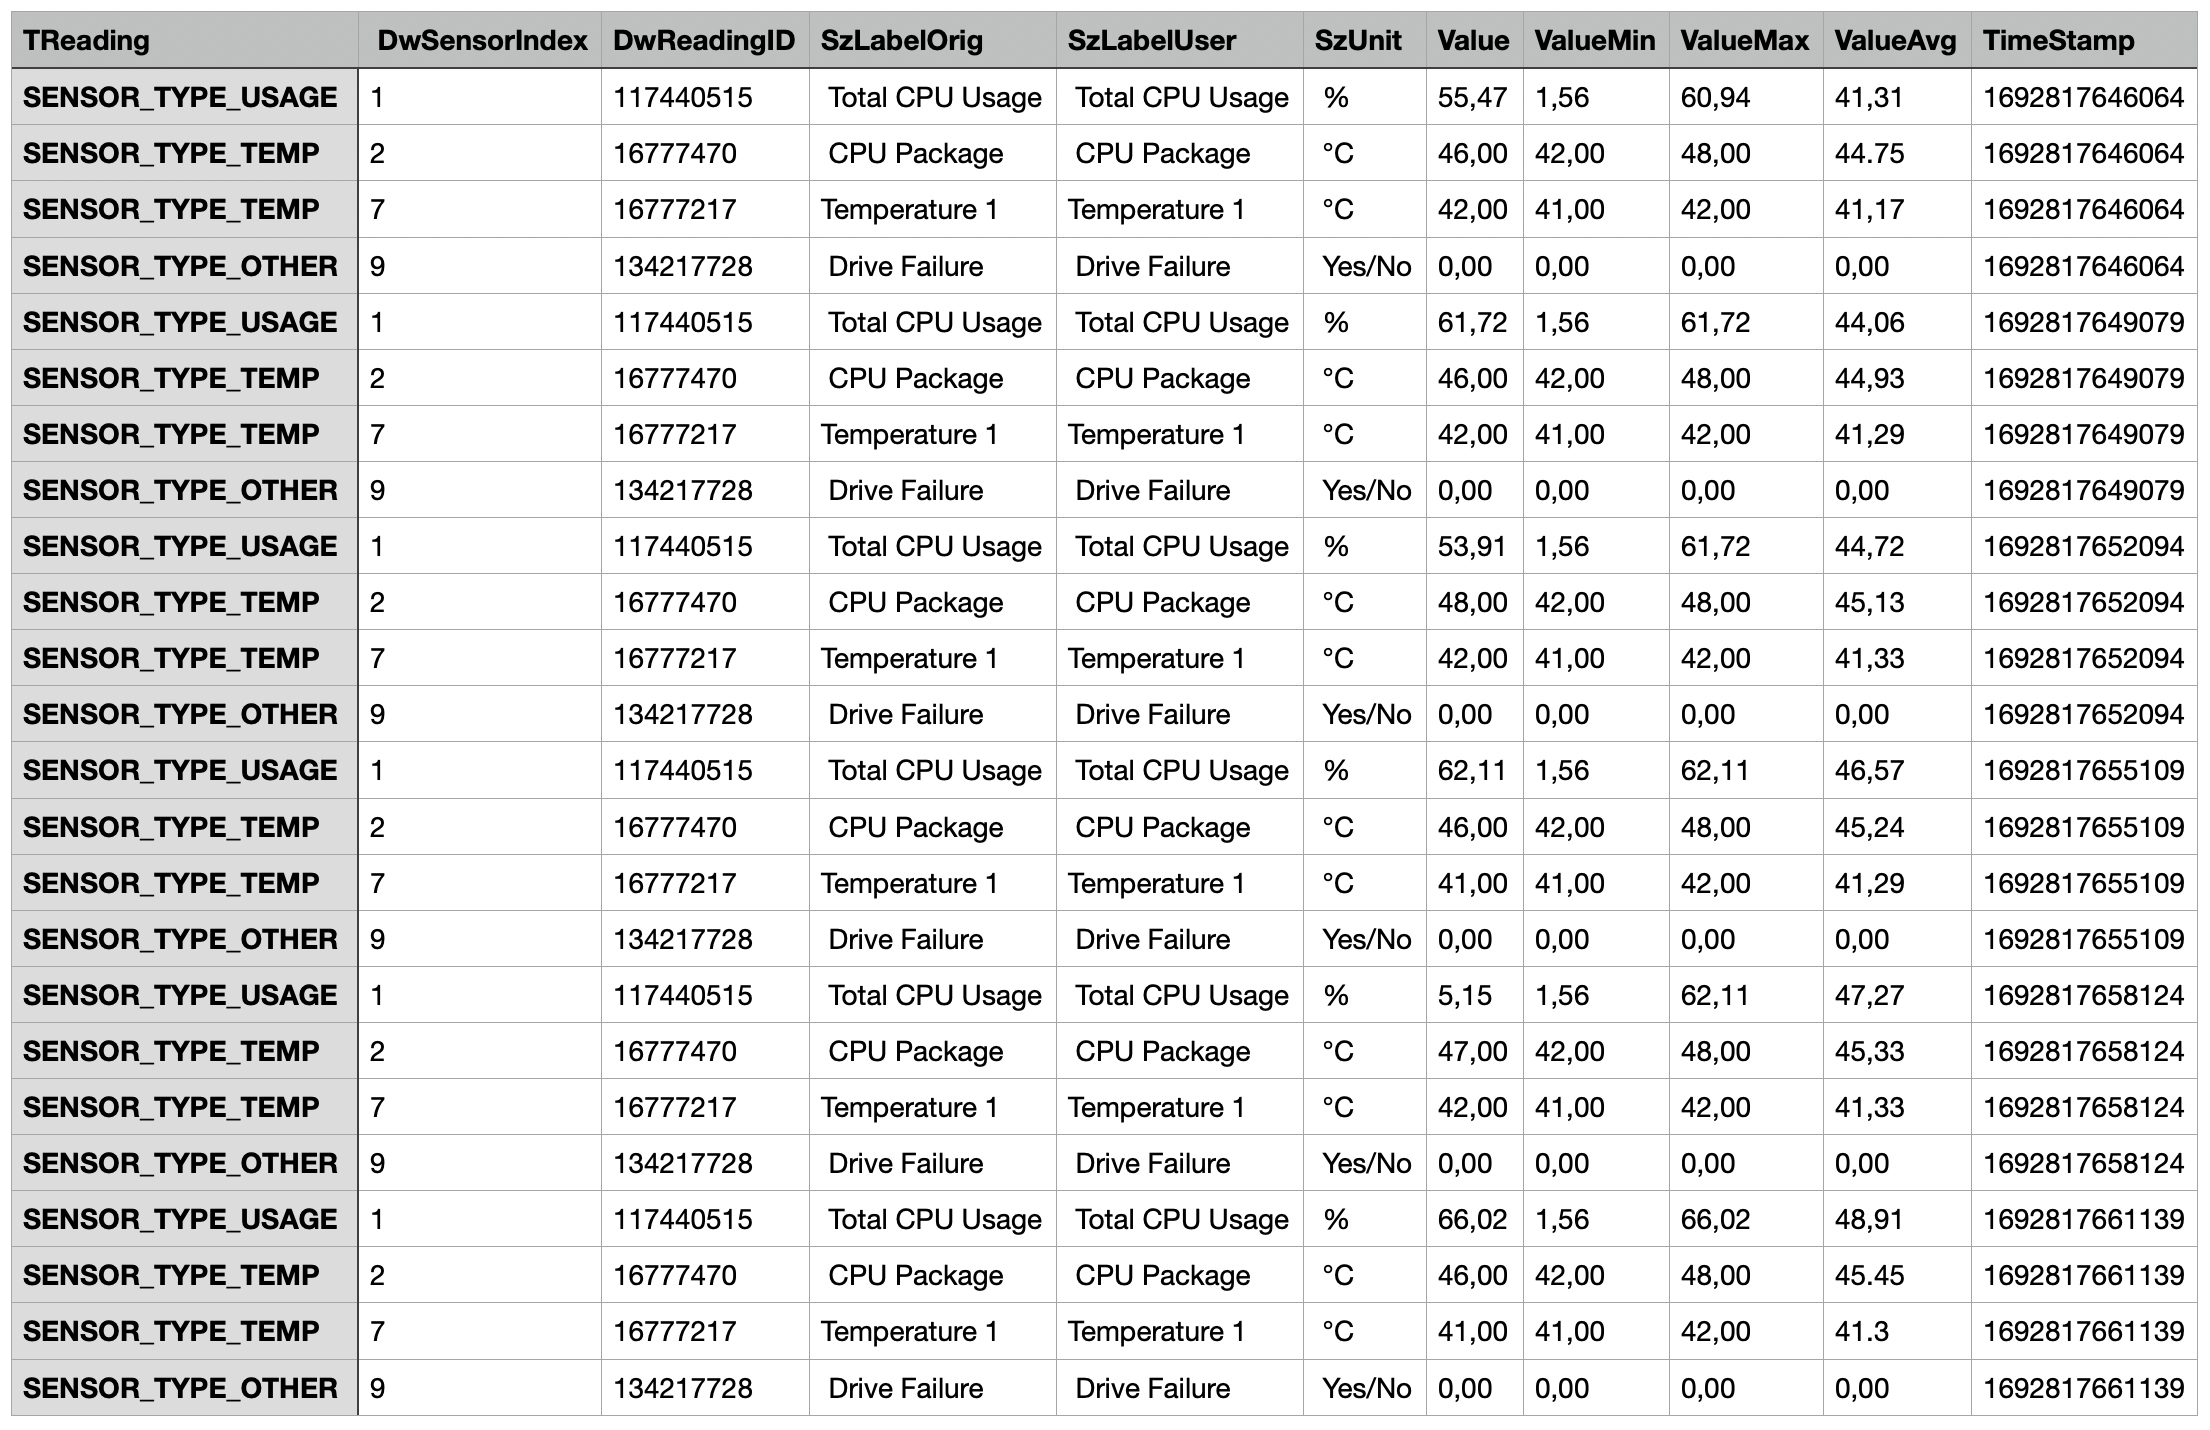
\includegraphics[width=0.81\textwidth]{SensorReadings.png}
        \caption{Beispiel einer Liste bestehend aus \textit{SensorData}}
        \label{fig:SensorReadings}
    \end{table}
\end{center}
\vspace{-1.8cm}
Da die \textit{HWiNFOWrapper} Schnittstelle alle verfügbraren Sensoren der VisuNet FLX Platform abdekt, ist die Strategie zum Auslesen dieser Platform recht Simpel. Dabei soll über einen Funktionsaufruf eine Liste mit den Aktuellen Messwerten der Sensoren erstellt und zurückgegeben werden.\\
Der \textit{ServiceControllerWrapper} liefert, neben dem werten des \textit{HWiNFOWrapper}, \ac{dpu} und \ac{tcu} Temperaturen der VisuNet GXP Platform. Die Datensätze der beiden Schnittstellen müssen daher in der \textit{GXPStrategy} kombiniert werden, sodas wie auch bei der \textit{FLXStrategy} jeweils eine Liste der Sensoren und eine Liste mit den Messwerten erstellt wird (Siehe Tabelle \ref{fig:SensorList} und \ref{fig:SensorReadings}).\\
Mithilfe der Strategieklassen kann somit für jegliche Hardwarekonfiguration einer Platform, eine gezielte Strategie erstellt werden, welche lediglich zwei Listen zurückliefert. Dabei ist der Anwendung selbst egal welche und wieviel Schnittstellen verwendet werden.

\subsection{Entwurf eines Datenbankmodells zum Speichern der Messwerte}
Im vorherigen Abschnitt \ref{sec:AuslesenHardware} wurde eine Architektur zum Auslesen der plattformunabhängigen Sensoren beschrieben. Resultierend daraus steht dem Programm eine Schnittstelle bereit, welche eine Reihe von Messdaten zur verfügung stellt. Ziel des Datenbankmodells ist es die bereitgestellten Messdaten in einem strukturierten und übersichtlichen Format ab zu speichern.\\
\subsubsection*{Zuordnung der Datensätze}
Aus Tabelle \ref{fig:SensorReadings} geht hervor das die Datensätze der SensorData Tabelle grundsätzlich in 3 kattegorien unterteilt werden können. Anhand der Spalte \textit{SzUnit} können die Daten in drei Kattegorien Temperatur (°C), Auslastung (\%) und Events (Yes/No) unterteilt werden. Bei weiterer Betrachtung der Datensätze wird zudem ersichtlich, das die Spalten \textit{TReading}, \textit{DwSensorIndex}, \textit{DwReadingID}, \textit{SzLabelOrig}, \textit{SzLabelUser} und \textit{SzUnit} bei jedem Sensor wiederholen.\\
Einhergehend aus diesen Beoabahtung wurde die in Abbildung \ref{fig:DBModell} abgebildete Struktur der Datenbank erstellt. 
\begin{center}
    \begin{figure}[h!]
        \centering
        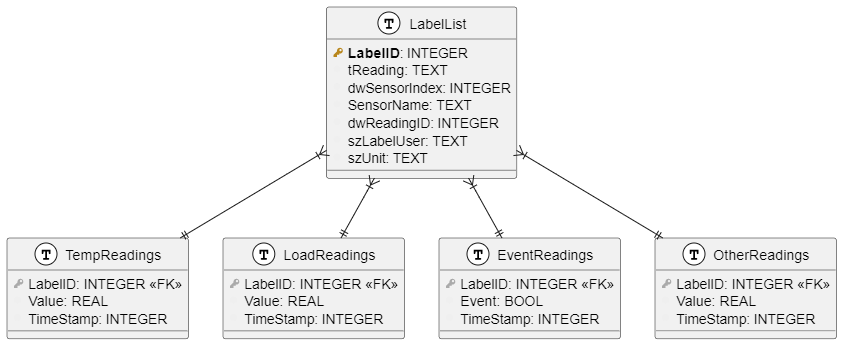
\includegraphics[width=1\textwidth]{DBModell.png}
        \caption{Datenbankmodell des Hardware-Health-Monitorings}
        \label{fig:DBModell}
    \end{figure}
\end{center}
\vspace{-1.8cm}
Die Datensätze der Tabellen \ref{fig:SensorList} und \ref{fig:SensorReadings} werden in 5 Datenbank Tabellen unterteilt. Dabei werden die Felder \textit{TReading}, \textit{DwSensorIndex}, \textit{DwReadingID}, \textit{SzLabel} und \textit{SzUnit} in die Tabelle \textit{LabelList} ausgelagert. Hinzu kommt das Feld \textit{SensorName}, welches aus Tabelle \ref{fig:SensorList} stammt. Über das Feld \textit{LabelID}, welches als Primär Schlüssel konfiguriert wird. Über diesen Schlüssel können nun die eigentlichen Messwerte, den Sensoren Zugeordnet werden. Die Messwerte werden dabei sortiert nach \textit{SzUnit} in vier Tabellen geschrieben. \textit{TempTabel} für Temperaturen in  °C, \textit{LoadReadings} für Auslastung in \%, \textit{EventTabel} für Events in 1/0 und \textit{OtherReadings} für alle andere Einheiten. Jede der vier Tabellen verfügt über ein Feld \textit{Value}, \textit{TimeStamp} und einer zugehörigen Schlüssel \textit{LabelID}.\\
Möchte man eine Reihe von messwerten eines Spezifischen Sensors erhalten, muss man zunächst den Primär Schlüssel des Sensors aus der \textit{LabelList} Tabelle ermitteln. Anschließend kann man die werte der entsprechenden Tabelle erhalten.
\subsubsection*{Erweiterung der Datenbank}
Zusätzlich zu den Ausgelesenen Messwerten, müssen auch die Ergebnisse der System Bewertung in der Datenbank abgelegt werden. 
Hierzu werden zunächst die Tabelle \textit{SystemStatus} und \textit{SystemMTBF} erstellt. Diese sind Identisch und unterscheiden sich lediglich in der Bedeutnug ihrer Werte. Der ermittelte Systemzustand wird in die Feldern \textit{Status}, \textit{Score} und \textit{Value} geschrieben. Die Felder \textit{TimeStampStart} und \textit{TimeStampEnd} grenzen das Interval, in welchem der Systemzustand ermittelt wurde ein. Des weiteren werden die Tabellen \textit{HistorySystemStatus} und \textit{SystemReliability} erzeugt. Diese Speichern die Historischen Werte des Systems, so wie dessen Verlässlichkeit ab. (Siehe Abbildung \ref{fig:DBModellErweitert})   
\begin{center}
    \begin{figure}[h!]
        \centering
        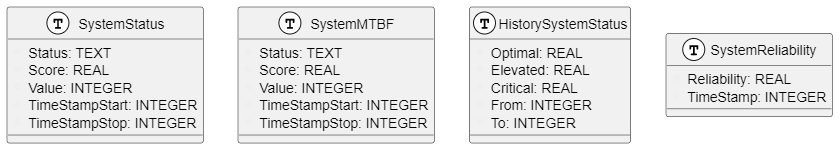
\includegraphics[width=1\textwidth]{DBErweitert.png}
        \caption{Datenbankmodellerweiterung des Hardware-Health-Monitorings}
        \label{fig:DBModellErweitert}
    \end{figure}
\end{center}
\vspace{-1.8cm}

\subsubsection*{Aufbau der Schnittstelle}\todo{Hier oder in die Implementierung und ConfigurationsDatei}
- komplizierte Syntax -> bedarf einer Abstraktion\\
- Datenbank wird über seperate Wrapperklasse ausgelesen und beschrieben. Hierzu Funktionen welche die datenbank beschreiben und auch wieder auslesen können. \\
- einführung der \textit{ValueReading}. Wird verwendet um eine Reihe von sensordaten abzu speichern. \\
- Funktionen zum auslesen bestimmter sensordaten, bezogen auf einen bestimmts intervall\\





















%===============================================================================
%Literaturverzeichnis
\addcontentsline{toc}{chapter}{Literaturverzeichnis}\printbibliography[title=Literaturverzeichnis]
\pagenumbering{Roman}
%Anhang

\end{document}
